% \abstract{ We discuss the problem of extending data mining
% approaches to cases in which data points arise in the form of
% individual graphs. Being able to find the intrinsic
% low-dimensionality in ensembles of graphs can be useful in a variety
% of modeling contexts, especially when coarse-graining the detailed
% graph information is of interest. One of the main challenges in
% mining graph data is the definition of a suitable pairwise
% similarity metric in the space of graphs. We explore two practical
% solutions to solving this problem: one based on finding subgraph
% densities, and one using spectral information. The approach is
% illustrated on three test data sets (ensembles of graphs); two of
% these are obtained from standard literature graph generating
% algorithms, while the graphs in the third example are sampled as
% dynamic snapshots from an evolving network simulation. We further
% combine these approaches with equation free techniques,
% demonstrating how such data mining can enhance scientific
% computation of network evolution dynamics.}

\section{\label{sec:intro} Introduction}

Microscopic, fine scale modeling and simulation is increasingly being
used to explore complex systems in fields such as epidemiology
\cite{Euba04modelling,Ferg05strategies,Long86predicting}, economics
\cite{Iori02microsimulation,Wang05microscopic}, biology
\cite{Levi01self-organization,Liu04stable}, and beyond.
% 
Network structures are key components of many such complex systems
\cite{Bara02linked:,Newm03structure}.  When the sizes of the networks
become large, it is important to find tools to systematically
reduce/analyze the networks.  In this paper, we will focus on the
issue of data mining, and the challenges involved in extending
standard data mining approaches to cases where every data point is a
graph.
% 
We also discuss the efficient estimation of various system properties
using data mining techniques, building significantly on previous work
\cite{rajendran2013analysis}.
% 

There are numerous applications in which data mining approaches on
graphs would be useful. They can be used to find the dimensionality of
the subspace in which any given collection of graphs lives. In other
words, data mining algorithms applied to collections of graphs can
help us understand the number of important variables required to
characterize (and thus parametrize) them. Being able to decipher the
minimum number of variables required to represent graphs is useful in
itself. One can then take the additional postprocessing step of
finding the relationship between variables extracted from data mining
and traditional network properties/descriptors. This {\em mapping}
from data-driven observables to ``typically used" observables is a
distinct, self-contained problem.

A separate class of problems in which data mining approaches can be of
crucial utility are those where the graph datasets come from a
dynamical process. In such cases, data mining can help us understand
the dynamics of the process. As before, in order to relate the data
mining results to actual properties of the system, one has to perform
additional postprocessing to map the data-driven observables to actual
system properties.
% 
We illustrate such methods on sets of graphs created by different
algorithmic processes in their full parameter space. This allows us to
estimate the dimensionality of the space in which these graphs live
i.e., to understand the actual variation in the graphs produced by
each of these algorithms, which is crucial in understanding whether
all the parameters in a model are independent.
% 
One can then seek ways to efficiently parameterize the graphs. To this
end, we address the independent issue of efficiently mapping between
the data-driven variables and the underlying network properties, and
use this to demonstrate how to accelerate the estimation of desired
dynamical quantities from the underlying process. This approach to
studying graph generating algorithms may also be used to propose and
test more generalized algorithms for generating graphs, that sample a
broader swath of the space of all possible graphs with a given
size. Such an algorithm can find use in parametric optimization
contexts, in helping to construct graphs with prescribed collective
properties \cite{Goun11generation}.

The paper is organized as follows: In Section \ref{sec:dm}, we briefly
discuss the data mining algorithm that will be used here. In Section
\ref{sec:sim}, we focus on the issue of defining similarities between
graphs, which is the biggest challenge in adapting traditional data
mining techniques to this context. In the same section, we also
discuss two options for solving this problem. We take three
illustrative examples and implement the data mining algorithm with our
two choices of similarity measures in Section ~\ref{sec:res}. In
Section ~\ref{sec: ef}, we discuss the mapping between the obtained
data mining variables and underlying properties of the network, also
providing an efficient method for the estimation of underlying
quantities of interest from a network-based dynamical system. A
summary of results and suggestions for future work are presented in
Section ~\ref{sec:conc}.

\section{\label{sec:dm}Data mining}

The ``traditional" tool in data mining is principal component analysis
(PCA) \cite{Shle03tutorial}, which is used to represent a low
dimensional dataset, embedded in high dimensional space, in terms of
the most meaningful linear basis. It enables one to identify
directions in which the data points have the most variance. But PCA is
only a linear analysis tool as it can only find out the best `linear'
lower dimensional subspace in which the dataset lives. In many
problems, the data lives in a highly \textit{non-linear} lower
dimensional subspace, making the necessary low dimensional
\textit{linear} subspace much higher dimensional compared to the true
dimensionality of the space in which the data lie. A number of
non-linear data mining tools such as Diffusion Maps
\cite{Nadl05diffusion,Nadl06diffusion} and ISOMAPs \cite{Tene00global}
are available to extract the non-linear subspace.  In this work, we
use Diffusion Maps as a representative non-linear data mining approach
in order to enable our discussion on extending these approaches to
ensembles of data where each data point is a graph.
% 
Diffusion maps (DMAPs) construct a graph whose vertices are the data
points (which in our case are each a graph); a similarity measure
between the data points is used as weights on the edges. In broad
terms, the eigenfunctions of the diffusion process on this graph are
used to embed the data points. If the data points actually lie in a
low dimensional non-linear subspace, the first few of these
eigenfunctions will be enough to embed the data and still be able to
recover the information about the it. A brief discussion of Diffusion
Maps is given below.

Consider a set of $n$ points $\{x_i\}_{i=1}^n \in \mathbb{R}^p$. We
define a similarity matrix, $W$ (which is a measure of closeness
between pairs of points in this space) as follows:

\begin{equation}
  W(i,j) = exp \left( \frac{-\|x_i-x_j\|^2}{\epsilon^2} \right).
  \label{eq:sim}
\end{equation}

% 
This is a Gaussian kernel. Here, $\epsilon$ is a suitable length scale
characterizing the immediate neighborhood of the point. Let us also
define a diagonal normalization matrix, $D_{ii}=\sum_j W_{ij}$, and
consequently the matrix, $A=D^{-1} W$. $A$ can be viewed as a Markov
matrix defining a random walk (or diffusion) on the data points, i.e.,
$A_{ij}$ denotes the probability of transition from $x_i$ to
$x_j$. Since $A$ is a Markov matrix, the first eigenvalue is always
$1$. The corresponding eigenvector is a constant, trivial
eigenvector. In diffusion maps, the next few non-trivial eigenvectors
of $A$ (corresponding to the next few largest eigenvalues) constitute
a useful parametrization of the non-linear subspace in which the data
lives. Thus, the leading DMap eigenvectors are used to characterize
this non-linear manifold.


As is evident in the description above, an important step in the
implementation of diffusion maps is the definition of the measure of
pairwise similarity between data points.
% 
If the data points live in a Euclidean space, it is straightforward to
use the Euclidean distance to measure the proximity pairs of data
points.
% 
When the data points are available in the form of graphs, however, it
is not trivial to define good measures of similarity between them.
% 
Thus, if all the machinery of non-linear data mining is to be
successfully adapted to the case of graph data, one has to be able to
define a measure of similarity and closeness between pairs of graphs.

\section{\label{sec:sim} Defining similarity measures between graph
  objects}

Although measures of similarity in the context of graphs have been
discussed in the literature \cite{Dana11algorithms}, complete
systematic classifications and definitions are still lacking.
% 
Firstly, one can either define similarities between nodes in a given
graph or similarities between the graphs themselves.
% 
In this paper, we will discuss the latter type, since we are
interested in comparing entire graph objects.
% 
Secondly, the nodes of the graphs can be labeled or unlabeled.
% 
We are interested here in the case of unlabeled nodes, where the
problem of ordering the nodes makes it more challenging to define
similarity measures.
% 
Additionally, we will focus on the case where all the graphs in the
dataset have the same number of nodes.
% 
However, the approach is, in principle, extendable to collections of
graphs of different sizes.
% 

Existing techniques in the literature for defining similarities may
roughly be classified into a few broad categories.
% 
The first of these is the class of methods that make use of the {\em
  structure} of the graphs to define similarities.
% 
% 
An obvious choice is to consider two graphs to be similar if they are
isomorphic \cite{Peli98replicator}.
% 
One of the first definitions of distance between pairs of graphs using
the idea of graph isomorphism was based on constructing the smallest
larger graph whose subset was isomorphic to both the graphs
\cite{Zeli75certain}.
% 
Likewise, one can define similarity measures based on the largest
common subgraph in pairs of graphs \cite{Bunk98graph,Raym02rascal:}.
% 
The graph edit distance, which measures the number of operations on
the nodes and edges of the graph required to transform one graph into
another, is another example of a method using the idea of graph
isomorphism.
% 
The graph edit distance and a list of other measures that use the
structure of the network to quantify similarity are defined in
\cite{Papa08web}.


% 
Next we have iterative methods that compare the behavior of the
neighborhoods of the nodes in the graphs.
% 
Comparing neighborhoods of nodes is especially applicable to measure
similarities between sparse graphs.
% 
Often, the graph similarity problem is solved through solving the
related problem of graph matching, which entails finding the
correspondence between the nodes in the two graphs such that the edge
overlap is maximal.
% 
Methods like the similarity flooding algorithm
\cite{Meln02similarity}, the graph similarity scoring algorithm
\cite{Zage08graph} and the belief propagation algorithm
\cite{Bay09message} are a few such approaches.
% 
Graph kernels based on the idea of random walks
\cite{Gaert03graph,Kash03marginalized,Mahe04extensions} also fall
under the category of algorithms based on comparing neighborhoods.

% 
However, one of the simplest options to evaluate similarities between
graphs is to directly compare a few chosen, representative features of
the network.
% 
The chosen features may correspond to any facet of the graph, such as
structural information (degree distribution, for instance) or spectral
measures (eigenvalues and/or eigenvectors of the graph Laplacian
matrix).
% 
In this paper, we will take this approach and consider two options for
defining similarities between graphs.
% 
The two options for defining similarity measures between graphs
considered here are: (i) using subgraph densities and (ii) an approach
using spectral information.
% 
A detailed description of the two proposed measures of graph
similarity follows.

\subsection{\label{ss:den} Subgraph density approach}

The general idea behind this approach is that two graphs are similar
if {\em the frequency of occurrence of representative subgraphs in
  these graphs is similar.}
% 
The density of a small subgraph in a large graph is a weighted
frequency of occurrence of the subgraph (pattern) in the large,
original graph.
% 
We use the following definition for the subgraph density of a subgraph
$H$ with $k$ nodes in a graph $G$ with $n$ nodes:

\begin{align}
  \label{eqn:homdenG}
  \rho(H,G) := \frac{1}{{n\choose k}} \!  \sum_{\varphi:[k] \to [n]} \!
  \left[ \forall  i, j \in [k] \! : \! H(i,j) \! = \! G_n(\varphi(i),
  \varphi(j)) \right].
\end{align}

% 
A graph can be reconstructed exactly if the densities of all possible
subgraphs onto the graph are specified \cite{Lov06limits}.
% 
Thus, a list of all these subgraph densities is an alternative way to
provide complete information about a graph.
% 
This list can be thought of as an embedding of the graph, which can
then be used to define similarity measures in the space of graphs.
% 
It is, however, not practical to find the subgraph densities of all
possible subgraphs of a given graph, especially when the number of
nodes in the graph becomes large.
% 
A systematic, yet practical, way to embed a graph is to use these
subgraph densities of all subgraphs lesser than a given size onto the
graph.
% 
For instance, to embed a graph with $n$ nodes, one can evaluate the
subgraph densities of all subgraphs of size less than or equal to
$m~(m \ll n)$.
% 
Since $m \ll n$, the embedding cannot be used to exactly reconstruct
the graph.
% 
One can, nevertheless, compute distances between the embeddings (the
vector of subgraph densities) of any two graphs and use them to
estimate similarities between these graphs.
% 

Let $G_i$ and $G_j$ be two graphs defined on $n$ nodes.
% 
Let $H_1$, $H_2$,$\ldots H_r$ be the $r$ chosen, representative
subgraphs.
% 
We find the frequencies of occurrence of these subgraphs in the
original graphs by appropriately modifying the open-source RANDESU
algorithm described in \cite{Wern06fanmod:}.
% 
The subgraph densities are calculated by dividing these frequencies by
$n\choose{k}$, where $n$ and $k$ are the number of nodes in the
original graph and the subgraph respectively.
% 
(Note that although dividing by $n\choose{k}$ is not a unique choice
for normalizing the subgraph densities, the densities we calculated
this way had similar orders of magnitude, and hence, this constitutes
a sensible choice.)
% 
The density of subgraph $H$ in graph $G$, denoted by $\rho(H,G))$, is
calculated as mentioned above.
% 
The similarity measure between a pair of graphs $G_i$ and $G_j$ can
then be defined as an $L_2$-norm (possibly weighted) of the difference
between two (finite) vectors of subgraph densities as follows:

\begin{equation}
  k(G_i,G_j) = \sqrt{\sum_{l=1}^{r}\left(\rho(H_l,G_i)-\rho(H_l,G_j)\right)^2}.
  \label{eq:k1}
\end{equation}

In order to use this pairwise similarity measure in a diffusion map
context, the Gaussian kernel, analogous to Eq.~\ref{eq:sim}, can be
calculated as follows:

\begin{equation}
  W(i,j) = exp \left( \frac{-(k(G_i,G_j))^2}{\epsilon^2} \right).
  \label{eq:sim1}
\end{equation}

In our illustrative numerical computations, we considered all
connected subgraphs of size less than or equal to $m=4$ as a
representative sample of subgraphs.
% 
There are $r=9$ such graphs as shown in Fig.~\ref{fig:SGs}.


\begin{figure}
  \begin{center}
    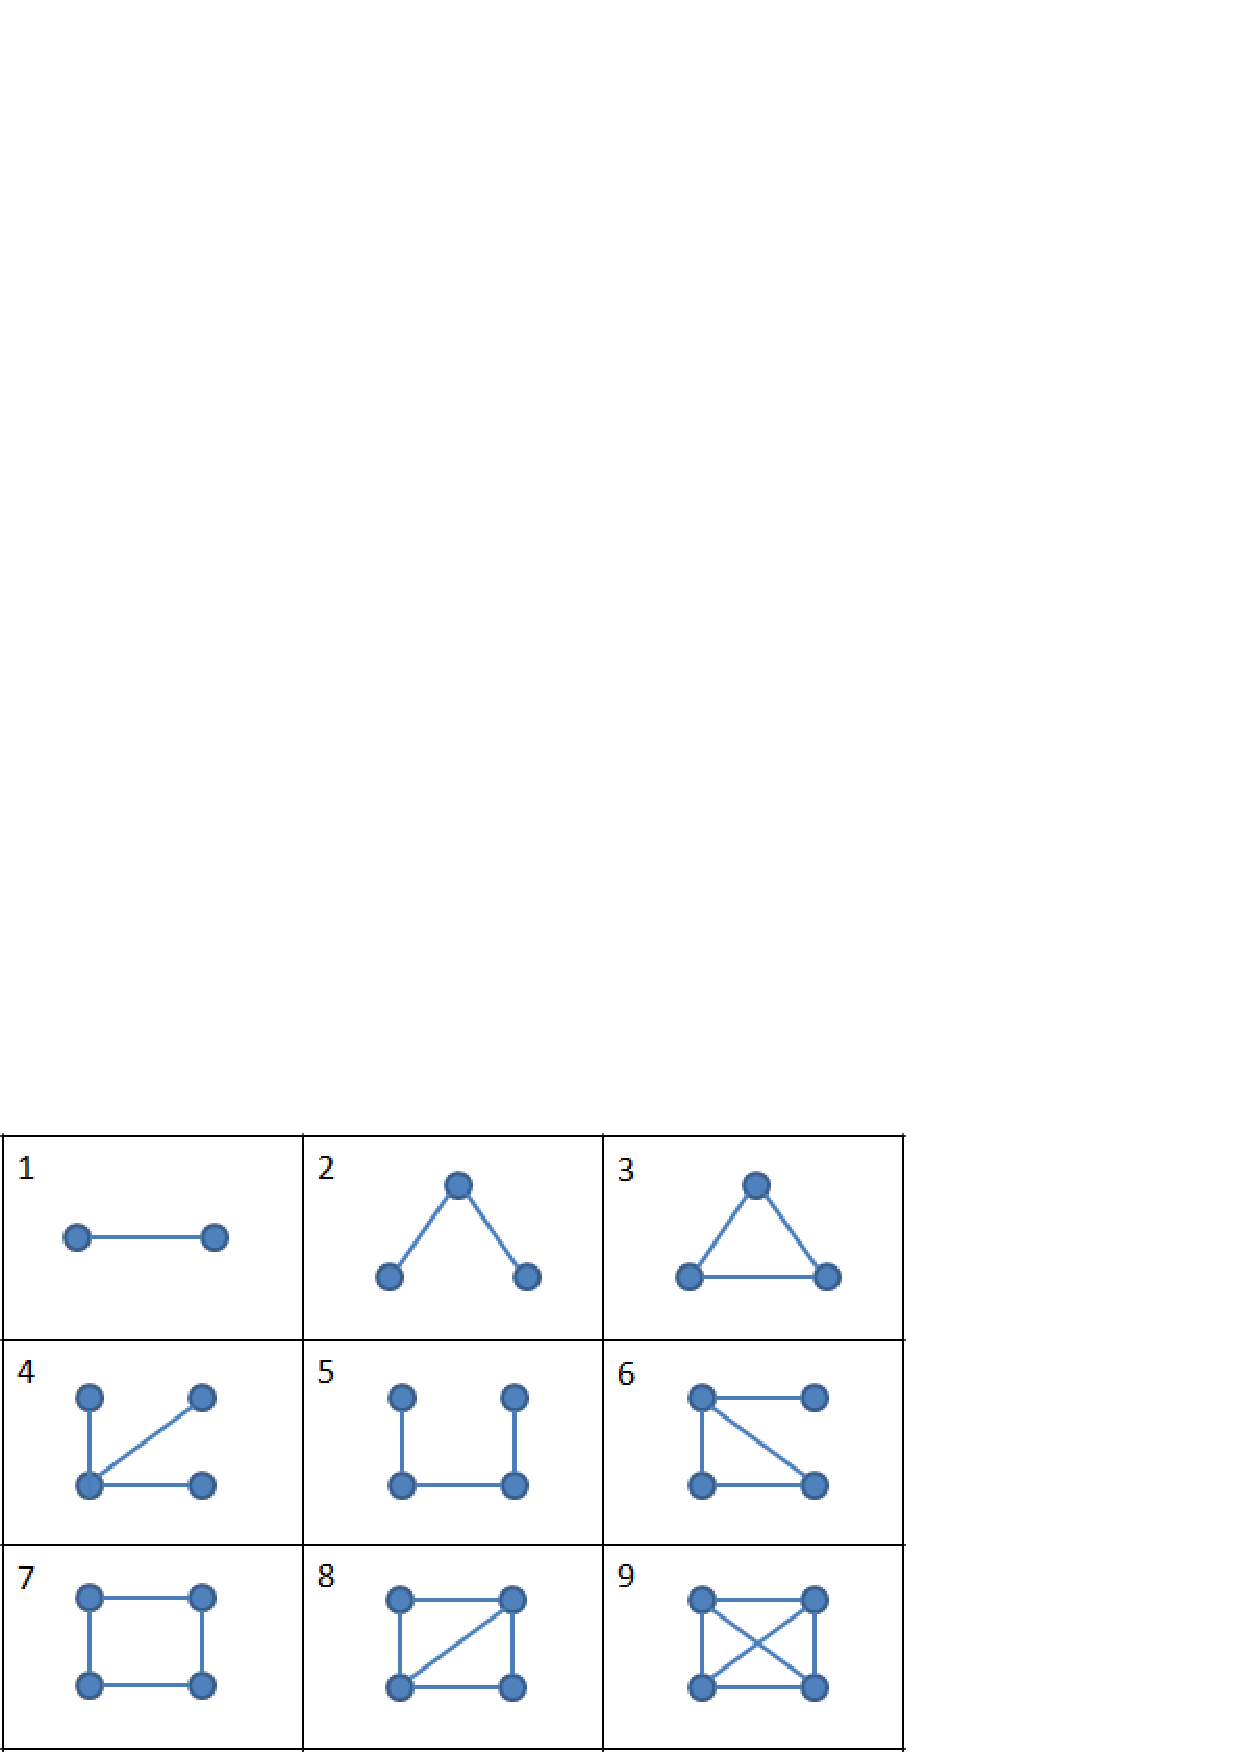
\includegraphics[width=0.63\textwidth]{SGs.pdf}
    \caption{\label{fig:SGs} The $9$ connected subgraphs of size less
      than or equal to $4$.  }
  \end{center}
\end{figure}


\subsection{\label{ss:s}Spectral approach}

Our second approach to defining similarities between graphs was
initially motivated by the approach given in \cite{Vis10graph}, and we
based it on the notion of non-conservative diffusion on graphs
\cite{Gho11non-conservative}.
% 
It has to be noted here that there are numerous ways in which the
spectral information of graphs (or equivalently information from
performing random walks on graphs) could be used to define similarity
measures.
% 
The particular version of the similarity metric discussed here is
inspired by the spectral decomposition algorithm in \cite{Vis10graph}.
% 
The usual definition of random walks on graphs is based on the
physical diffusion process.
% 
One starts with a given initial density of random walkers, who are
then redistributed at every step by premultiplying the distribution of
random walkers at the current stage by the adjacency matrix.
% 
The rows of the adjacency matrix are scaled by the row sum so that the
quantity of random walkers is conserved.
% 
In our approach, we consider a non-conservative diffusion process,
where we replace the normalized adjacency matrix in the random walk
process by its original, unnormalized counterpart.


Let us consider two graphs $G_i$ and $G_j$, with adjacency matrices
$B_i$ and $B_j$ respectively.
% 
Let their spectral decompositions be given by $B_i = P_i D_i P_i^{T}$
and $B_j = P_j D_j P_j^{T}$ respectively.
% 
% 
Let the initial probability distribution of random walkers on the $n$
nodes of the graph be denoted by $\hat{p}$.
% 
This can be taken to be a uniform distribution.
% 
At every step of the process, the new distribution of random walkers
is found by applying the unnormalized adjacency matrix to the
distribution at the previous step.
% 
Since the adjacency matrix is not normalized, the density of random
walkers change over time depending on the weights associated with the
edges of the graphs.
% 
We consider walks of different lengths, at the end of which we
evaluate statistics by weighing the density of random walkers on the
nodes according to vector $\hat{q}$, which can also be assumed to be a
uniform vector that takes the value $1/n$ corresponding to every node.
% 
As pointed out in \cite{Vis10graph}, the vectors $\hat{p}$ and
$\hat{q}$ are ways to \emph{``embed prior knowledge into the kernel
  design"}.
% 
Although the method is general, we will consider the special case
where the sizes of the graphs are the same.


The (possibly weighted) average density of random walkers after a
k-length walk in $G_i$, denoted by $Q_{ik}$.
% 
This can be evaluated as follows:

\begin{equation}
  Q_{ik} = \hat{q}^\mathrm{T}B_i^k \hat{p} = \hat{q}^\mathrm{T} (P_i D_i^k P_i^{T}) \hat{p}.
\end{equation}

Consider a summation of $Q_{ik}$ for walks of all lengths with
appropriate weights $\mu_k$ corresponding to each value of $k$.
% 
Where $l_i=P_i^\mathrm{T}\hat{q}$ and $r_i=P_i^{T} \hat{p}$, let the
computed weighted sum of densities corresponding to graph $G_i$ be
denoted as $S_i$:

\begin{equation}
  S_i = \sum_{k=0}^{\infty} \mu(k) Q_{ik} = \sum_{k=0}^{\infty} \mu(k)~l_i^\mathrm{T} D_i^k r_i.
\end{equation}

We used the following choice of weighting relation:
$\mu(k) = \frac{\lambda^k}{k!}$.
% 
With this choice of weights, one can write $S_i$ as a simple function
of $\lambda$ as follows:

\begin{equation}
  S_i(\lambda) = l_i^\mathrm{T}e^{(\lambda D_i)}r_i.
  \label{eq:S}
\end{equation}

Thus, every graph $G_i$ is embedded using these $S_i$ values evaluated
at characteristic values of $\lambda$ (say
$\lambda_1, \lambda_2,... \lambda_M$)\footnote{Note that an
  alternative equivalent way to define the similarity measure would be
  to directly compare the contribution of the different eigenvectors
  to $S_i$ instead of summing the contributions and then using
  different values of $\lambda$.  However, it is difficult to
  generalize this approach to cases where there are graphs of varying
  sizes.}.
% 
The similarity between any two graphs $G_i$ and $G_j$ can then be
evaluated using the Gaussian kernel defined in Eq.~\ref{eq:sim1} using
the following expression for $k(G_i,G_j)$:

\begin{equation}
  k(G_i,G_j) = \sqrt{\sum_{m=1}^{M} (S_i(\lambda_m)-S_j(\lambda_m))^2}.
  \label{eq:k2}
\end{equation}

This formula is very convenient for our purpose.
% 
For every graph $G_i$, one can evaluate the three vectors, $l_i$,
diagonal elements of $D_i$ and $r_i$ and store them.
% 
These $3n$ numbers can be thought of as a coarse embedding of the
graph.
% 
The similarity measure between pairs of graphs can finally be
evaluated by using Eq.~\ref{eq:S} and Eq.~\ref{eq:k2} by substituting
in these stored values.
% 
This also makes it easier to add new graphs and increase the size of
the similarity matrix without having to do too much additional
computation.
% 

\section{\label{sec:res} Computational results}


We will explore the dimensionality of datasets (where the data points
are individual graphs) using the diffusion map approach; within this
approach we will construct implementations using the graph similarity
metrics mentioned above.
% 
We use three different datasets for this exploration; two of them
arise in the context of ``graph-generation" models (they are the
ubiquitous Erd\"{o}s-R\'{e}nyi networks and the Chung-Lu networks).
% 
The third is closer to the types of applications that motivated our
work: networks that arise as individual temporal ``snapshots" during a
dynamic network evolution problem.
% 
% For each example, we will use both the subgraph and the spectral
% approaches described here to quantify the similarities between pairs
% of graphs.
% 

\subsection{\label{ss:er} Test case $1$: Erd\"{o}s-R\'{e}nyi graphs}

\begin{figure}
  \begin{center}
    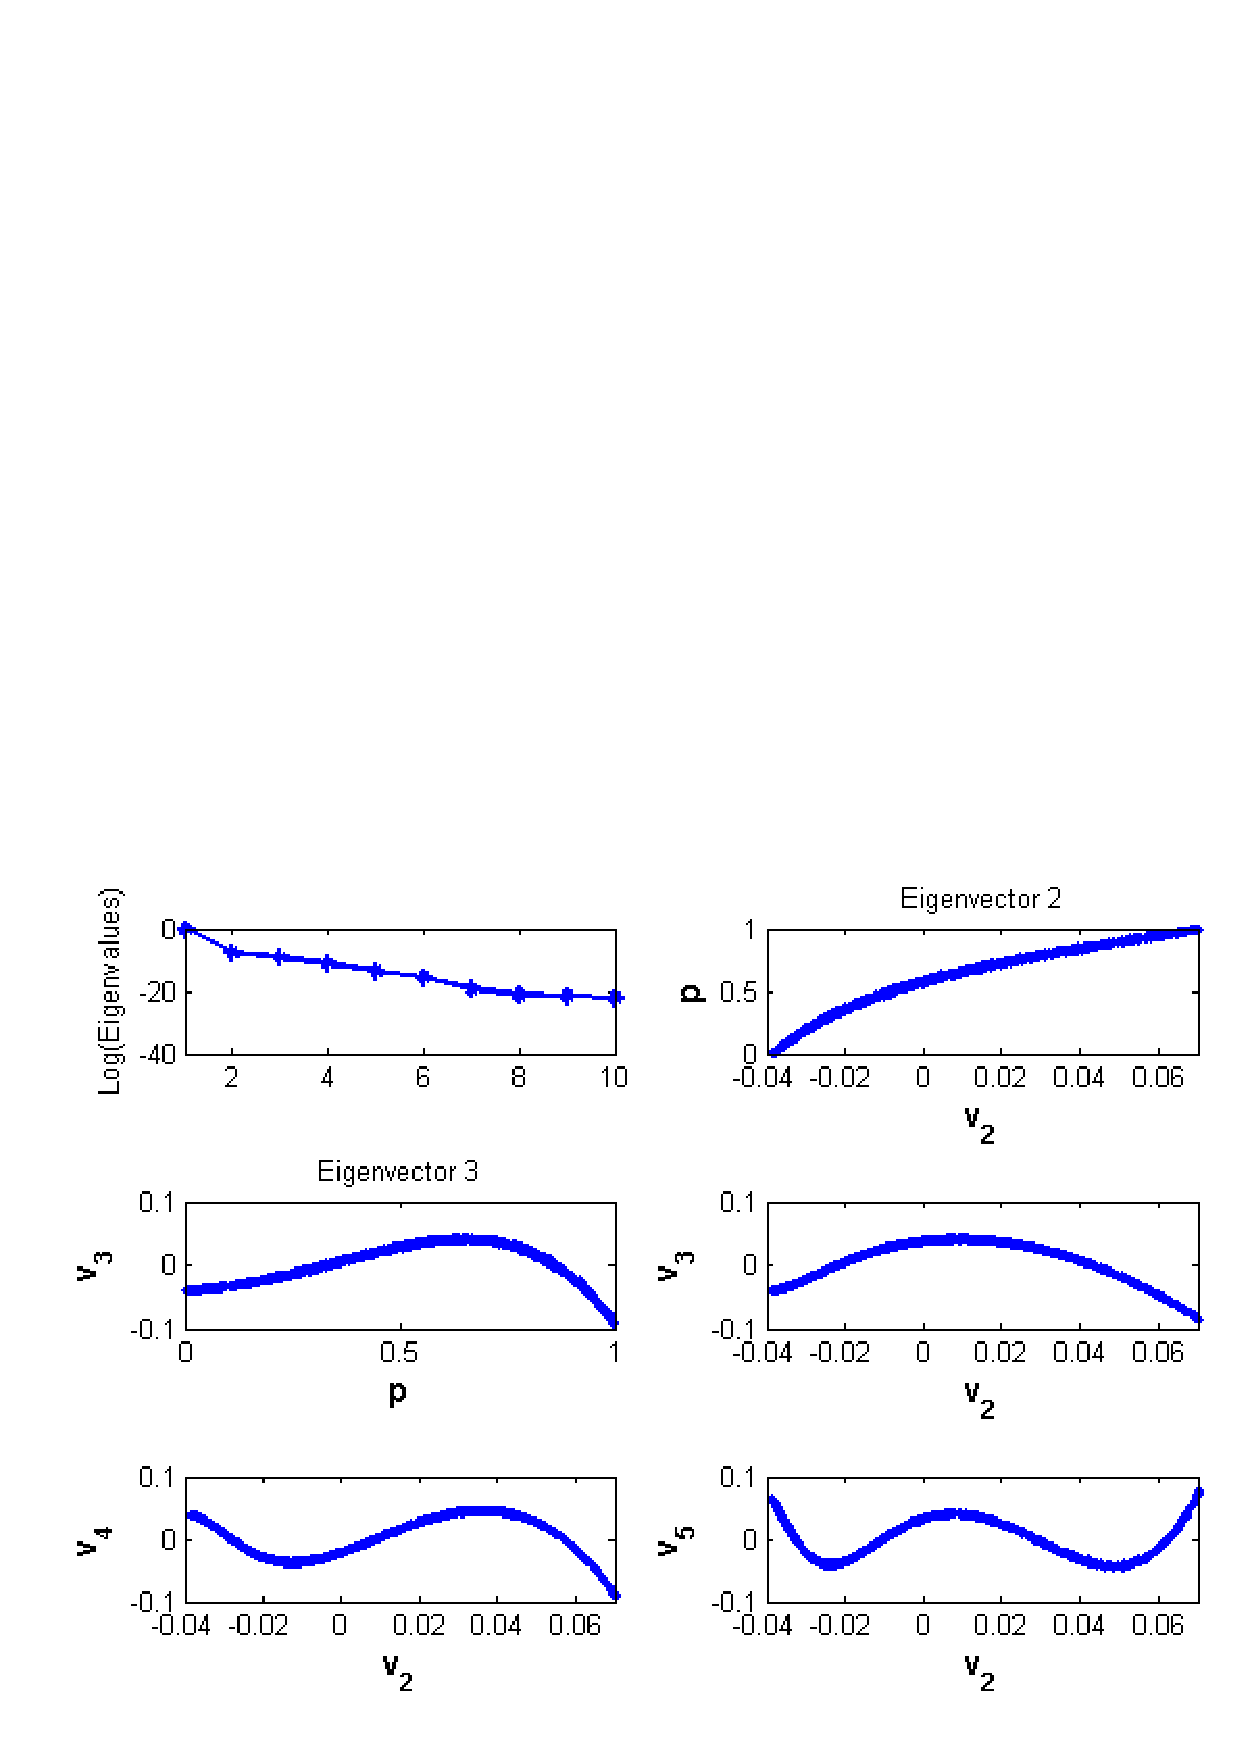
\includegraphics[width=0.81\textwidth]{ER1_ev.pdf}
    \caption{\label{fig:ER1} Data mining ensembles of
      Erd\"{o}s-R\'{e}nyi graphs: The subgraph approach was used to
      quantify similarity between individual graphs (see text).  The
      top-left plot shows the first $10$ eigenvalues of the random
      walk matrix arising in Diffusion Maps.  The corresponding first
      two non-trivial eigenvectors are plotted against the
      ``construction parameter" $p$ used to create the graphs, as well
      as against each other.  Notice how the first non-trivial
      eigenvector (the second eigenvector) is one-to-one with $p$.  }
  \end{center}
\end{figure}

\begin{figure}
  \begin{center}
    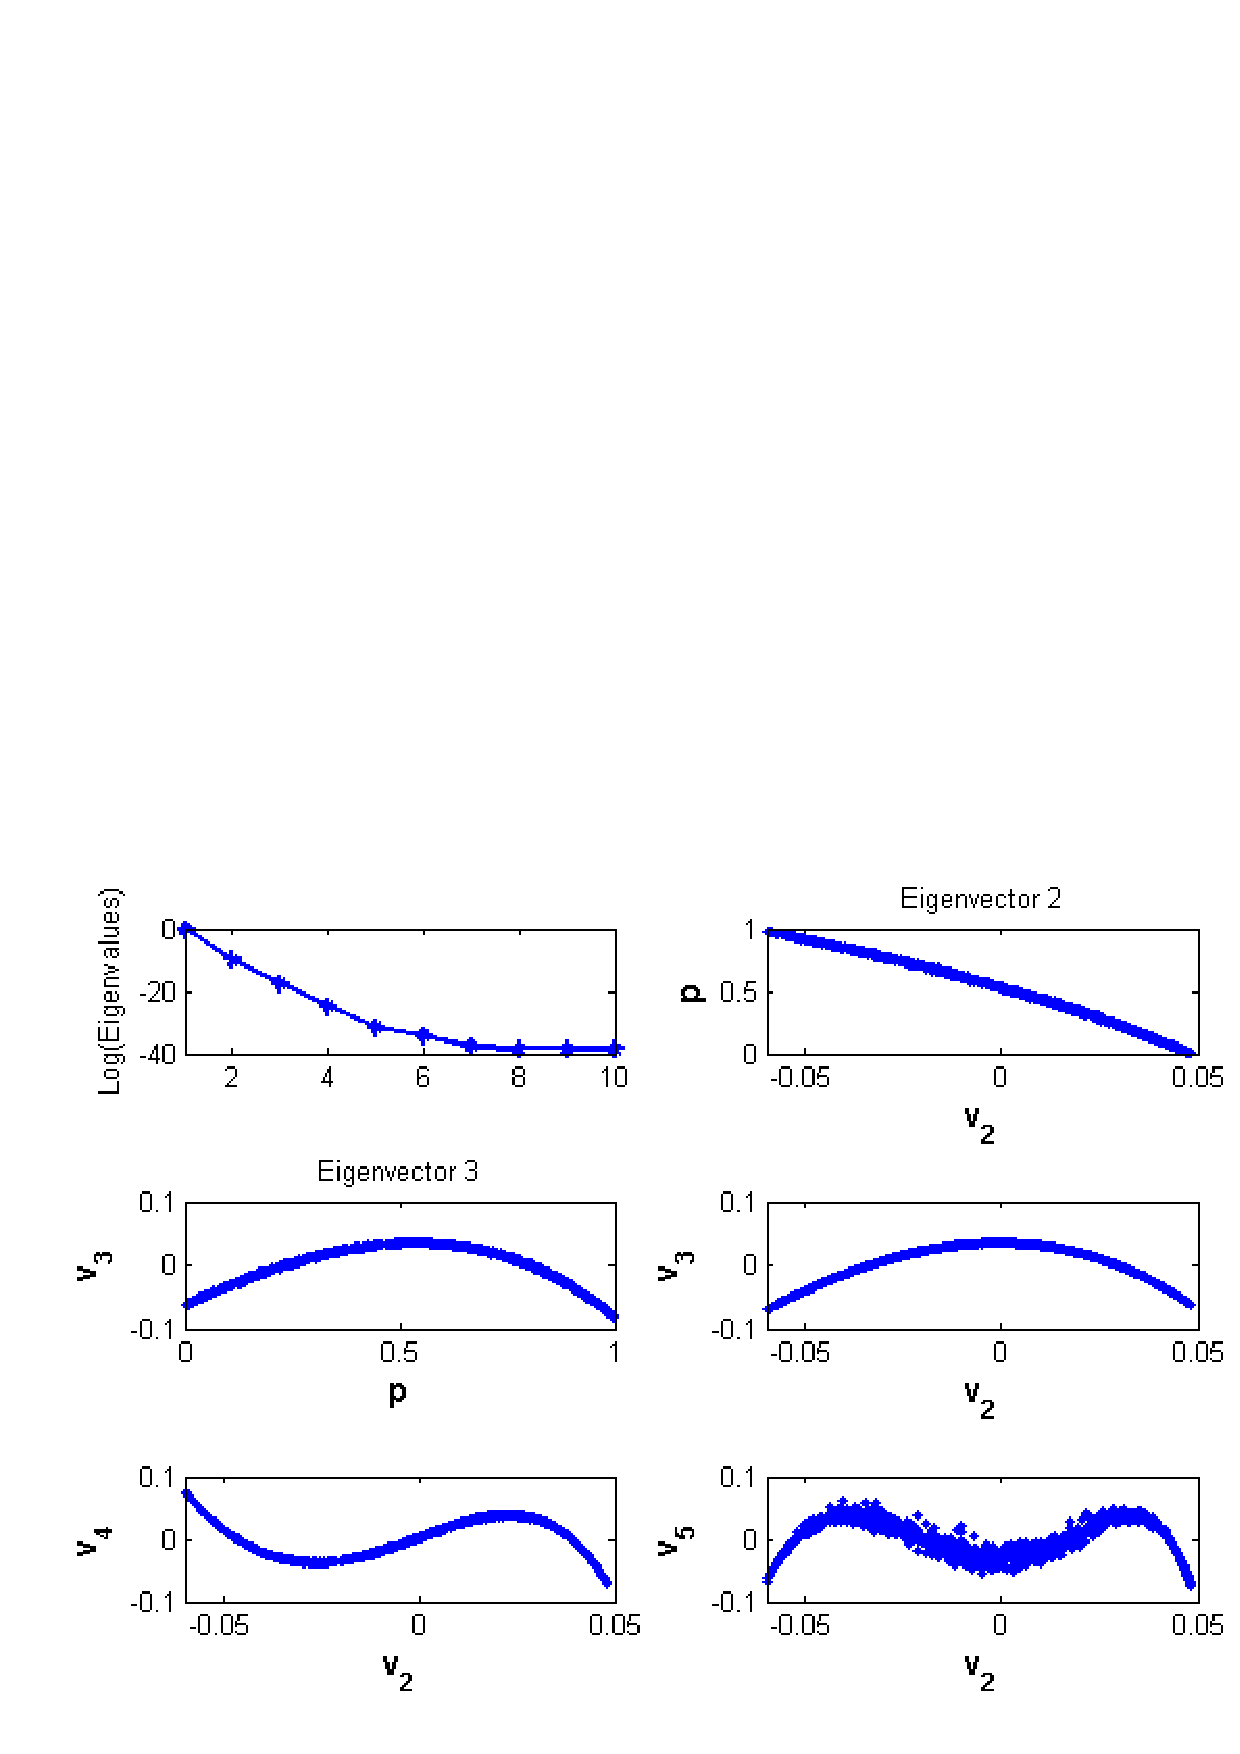
\includegraphics[width=0.81\textwidth]{ER2_ev.pdf}
    \caption{\label{fig:ER2} Data mining ensembles of
      Erd\"{o}s-R\'{e}nyi graphs: Our spectral approach was used to
      quantify similarity between graphs (see text). The top-left plot
      shows the first $10$ eigenvalues of the random walk matrix
      arising in Diffusion Maps. The corresponding first two
      non-trivial eigenvectors are plotted against the construction
      parameter $p$ used to create the graphs, as well as against each
      other.  Notice how, again, the first non-trivial eigenvector
      (the second eigenvector) is one-to-one with $p$.  }
  \end{center}
\end{figure}


Consider, as our initial example, a dataset consisting of $m=1000$
Erd\"{o}s-R\'{e}nyi $G(n,p)$ random graphs \cite{Erd59random} with
$n=100$ nodes each.
% 
The parameter $p$ (the probability of edge existence) used to
construct these graphs is randomly sampled uniformly in the interval
$(0,1)$.
% 
The diffusion maps algorithm is then applied on this set of graphs.
% 
We start by computing the similarity measures between pairs of
individual graphs (both the subgraph (Eq.~\ref{eq:k1}) -using $9$
subgraph densities- and our spectral approach (Eq.~\ref{eq:k2} -using
100 $\lambda$ values-).
% 
The similarity matrix $W$ is then calculated using Eq.~\ref{eq:sim1}.
% 
The first $10$ eigenvalues of the corresponding random walk matrix
$A$, (as described in Sec.~\ref{sec:dm}) are plotted in
Figs.~\ref{fig:ER1} and \ref{fig:ER2}, corresponding to the subgraph
and to our spectral approach respectively.
% 
For both these cases, the first two non-trivial eigenvectors (viz.,
the eigenvectors corresponding to the second and third eigenvalues)
are plotted against the parameter $p$ of the corresponding
Erd\"{o}s-R\'{e}nyi graph.
% 
From the figures, it is clear that the second eigenvector is
one-to-one with the parameter $p$, which here is also the
edge-density.
% 
Thus, this eigenvector (in both cases) captures the principal
direction of variation in the collection of Erd\"{o}s-R\'{e}nyi
graphs.
% 
In other words, our data mining approach independently recovers the
single important parameter $p$ in our sample dataset.
% 

As these Erd\"{o}s-R\'{e}nyi graphs can be parameterized using just a
single parameter $p$, one might expect a gap in the eigenspectrum
after the second (first nontrivial) eigenvalue, and also expect the
remaining eigenvalues/vectors to correspond to some sort of ``noise":
the variability of sampling among Erd\"{o}s-R\'{e}nyi graphs of the
same $p$.
% 
Interestingly, no such gap can be observed in our plots after the
second eigenvalue.
% 
If, however, subsequent eigenvectors are plotted against the second
one on our data, we clearly observed that they are simply higher
harmonics in "the same dimension".
% 
The third, fourth and fifth eigenvectors, in both cases, are clearly
seen to be a non-monotonic function of $v_2$($p$) but with an
increasing number of ``spatial" oscillations, reminiscent of
Sturm-Liouville type problem eigenfunction shapes.
% 
These eigenvectors do not, therefore, capture new directions in the
space of our sample graphs.
% 
% The same holds true for several higher eigenvectors as well

This simple example serves to illustrate the purpose of using data
mining algorithms on graph data.
% 
In this case, we created a one parameter family of graphs,
characterized by the parameter $p$.
% 
Using only the resulting graph objects, our data mining approach
successfully recovered a characterization of these graphs equivalent
to (one-to-one with) this parameter $p$.
% 
One feature of this one-to-one correspondence between $p$ and the
$v_2$ component of the graphs is worth more discussion: data mining
discovers the ``one-dimensionality" of the data ensemble, but does not
{\em explicitly} identify $p$ - a parametrization that has a direct
and obvious physical meaning.
% 
Data mining only provides a parametrization effectively isomorphic to
the one by $p$: to the eye the $p$-$v_2$ function appears continuous
and with a continuous inverse.
% 
Providing a physical meaning for the parameterization discovered (or
finding a physically meaningful parameterization isomorphic to the one
discovered) is a distinct task, where the modeler is expected to
provide good candidates.
% 
The contribution of the data-mining process is determining the {\em
  number} of necessary parameters, and in providing a quantity against
which good candidates can be tested.


\subsection{\label{ss:cl} Test case $2$: A two parameter family of
  graphs}

\begin{figure}
  \begin{center}
    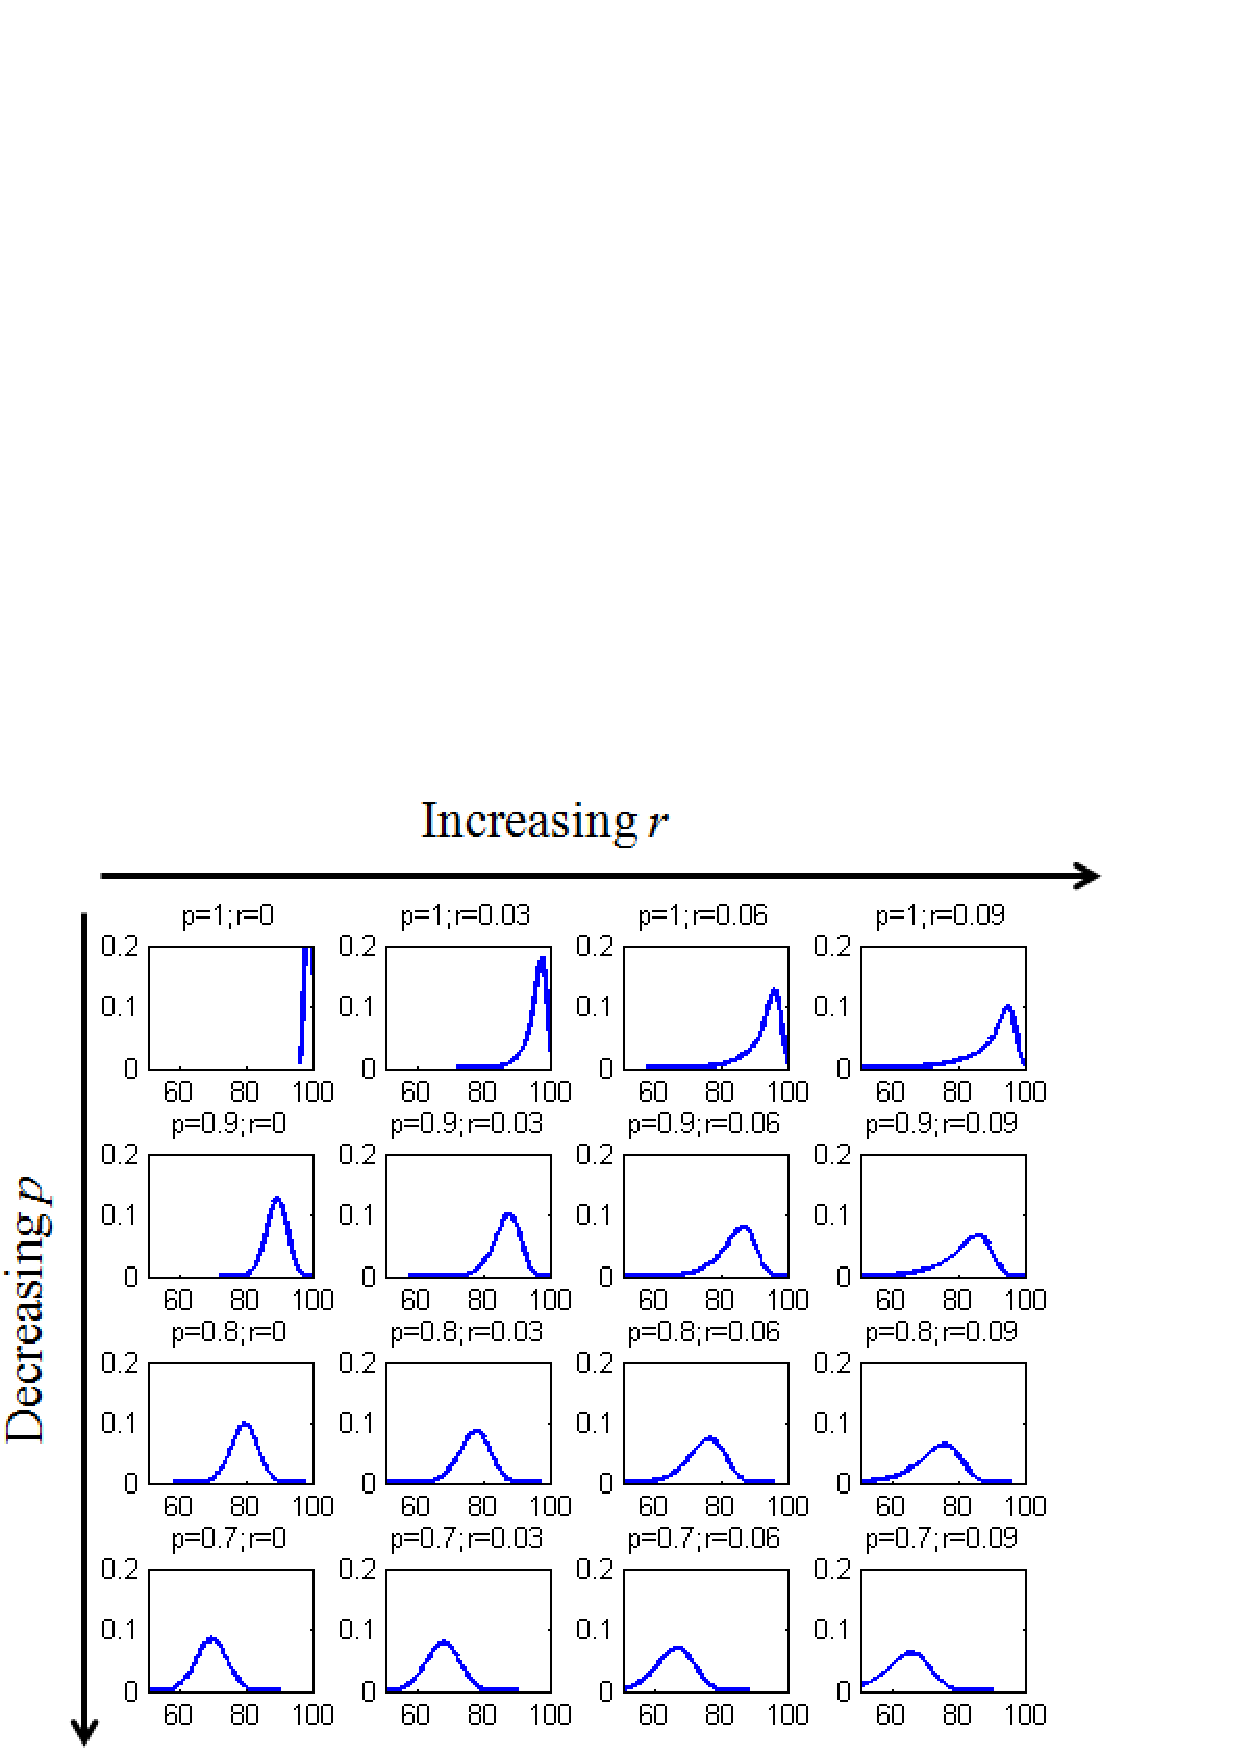
\includegraphics[width=0.81\textwidth]{CL_dd.pdf}
    \caption{\label{fig:CL} The degree distribution of Chung-Lu graphs
      created using the algorithm described in the text are plotted
      for various values of the construction parameters $p$ and
      $r$. The parameter $p$ corresponds to the density of edges in
      the graph. As $p$ decreases, the degree distribution shifts
      uniformly to the left.  The parameter $r$ corresponds roughly to
      the skewness of the degree distribution.  As $r$ is increased
      from $0$, the degree distribution shifts to the left, and
      resulting degree distributions are skewed more and more to the
      left.  }
  \end{center}
\end{figure}


\begin{figure}
  \begin{center}
    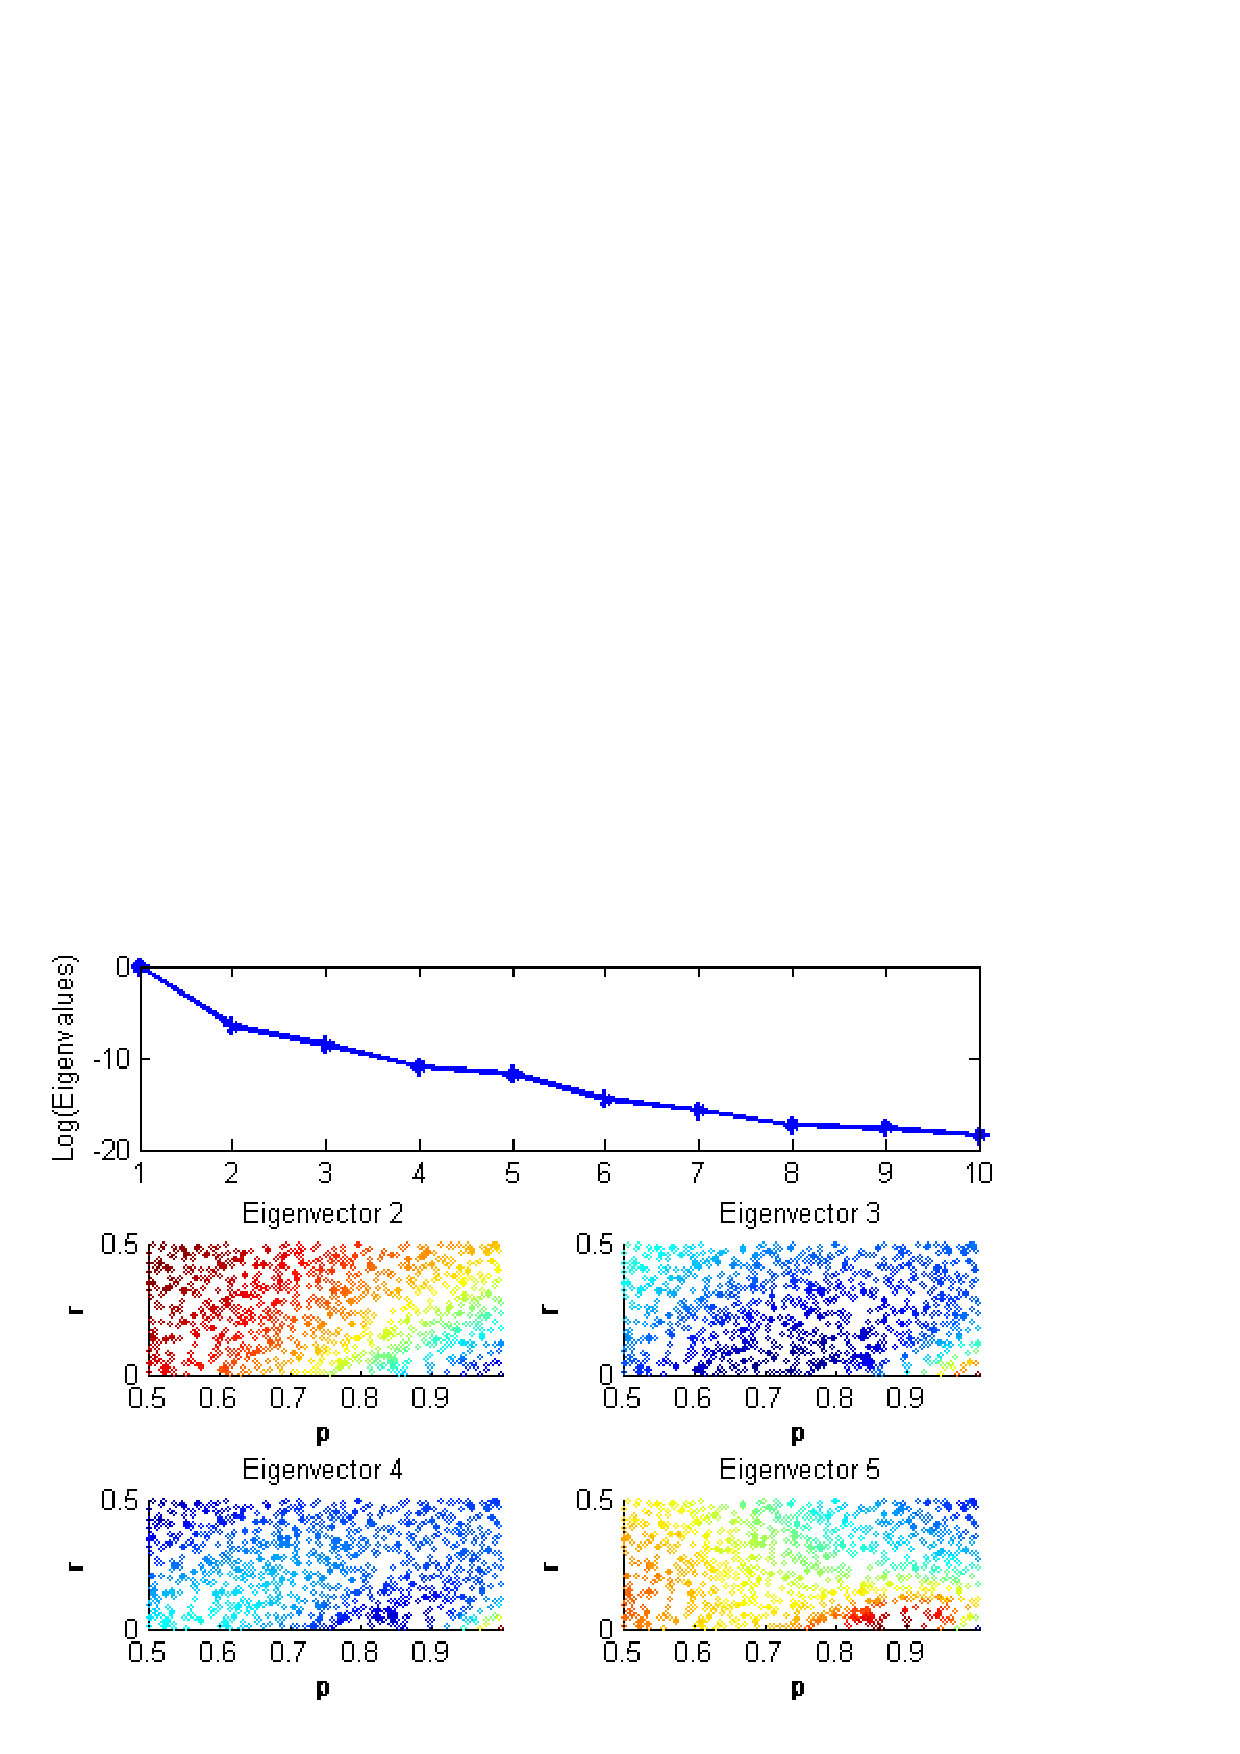
\includegraphics[width=0.81\textwidth]{CL1_ev.pdf}
    \caption{\label{fig:CL1} Data mining ensembles of two-parameter
      Chung-Lu graphs: The leading eigenvalues of the random walk
      matrix calculated using the subgraph similarity measure are
      first plotted.  The corresponding first four non-trivial
      eigenvectors are then illustrated in a way that brings forth
      their relation to the construction parameters $p$ and $r$.  In
      these plots, each graph is denoted as a point.  The $x$ and $y$
      coordinates of the point correspond to the parameters $p$ and
      $r$ used to construct that particular graph.  The graphs are
      colored based on the magnitude of their components in the
      eigenvectors of the random walk matrix $A$.  }
  \end{center}
\end{figure}

\begin{figure}
  \begin{center}
    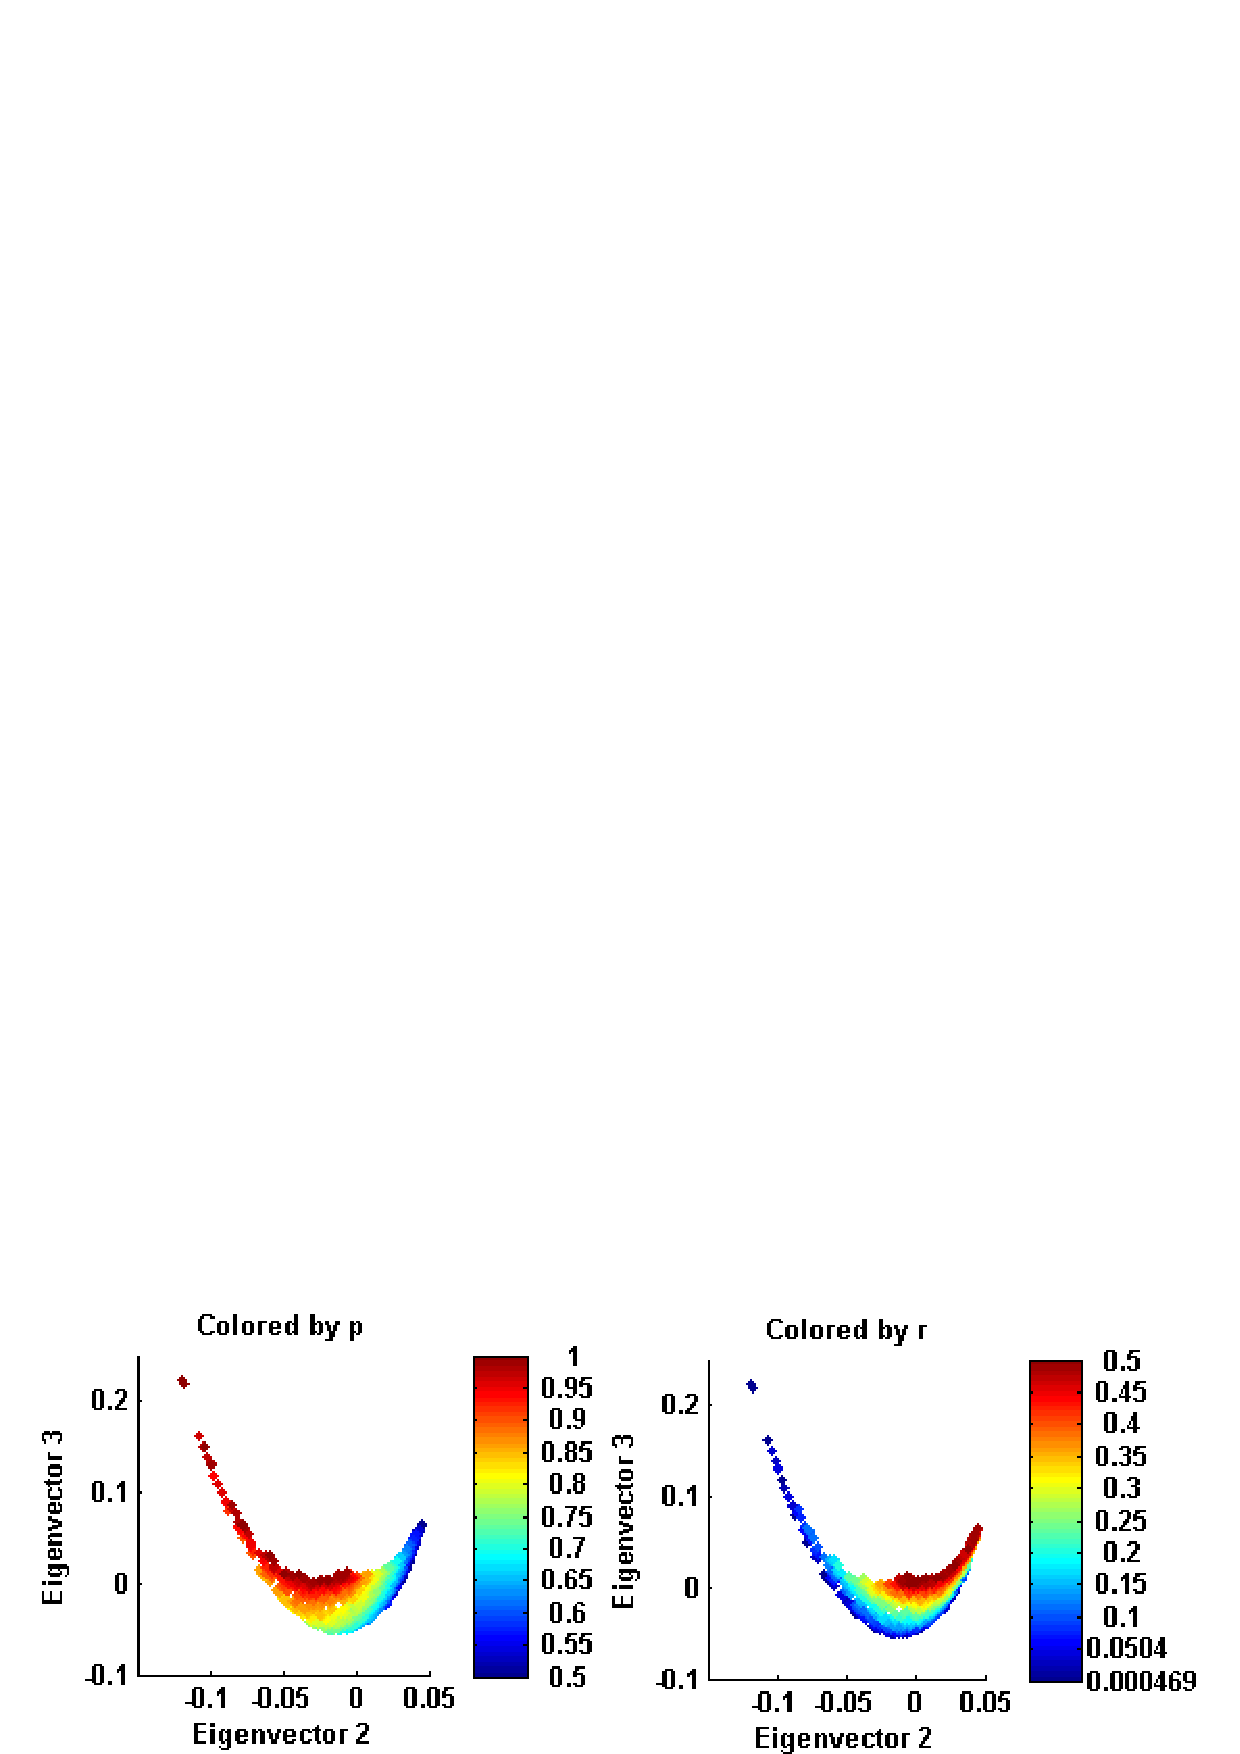
\includegraphics[width=0.81\textwidth]{CL1a.pdf}
    \caption{\label{fig:CL1a}
      Data mining the two-parameter family of Chung-Lu graphs using the subgraph similarity metric
      leads to an apparent two-dimensional
      embedding.
      % 
      In these plots the $x$ and $y$ coordinates of each point (i.e. of each graph in the dataset)
      denote the components
      of that particular graph in the second and third eigenvectors of the random walk matrix respectively.
      % 
      Each point is now colored based on the parameter values of $p$
      (left) and $r$ (right) used to construct the particular graph.
    }
  \end{center}
\end{figure}

\begin{figure}
  \begin{center}
    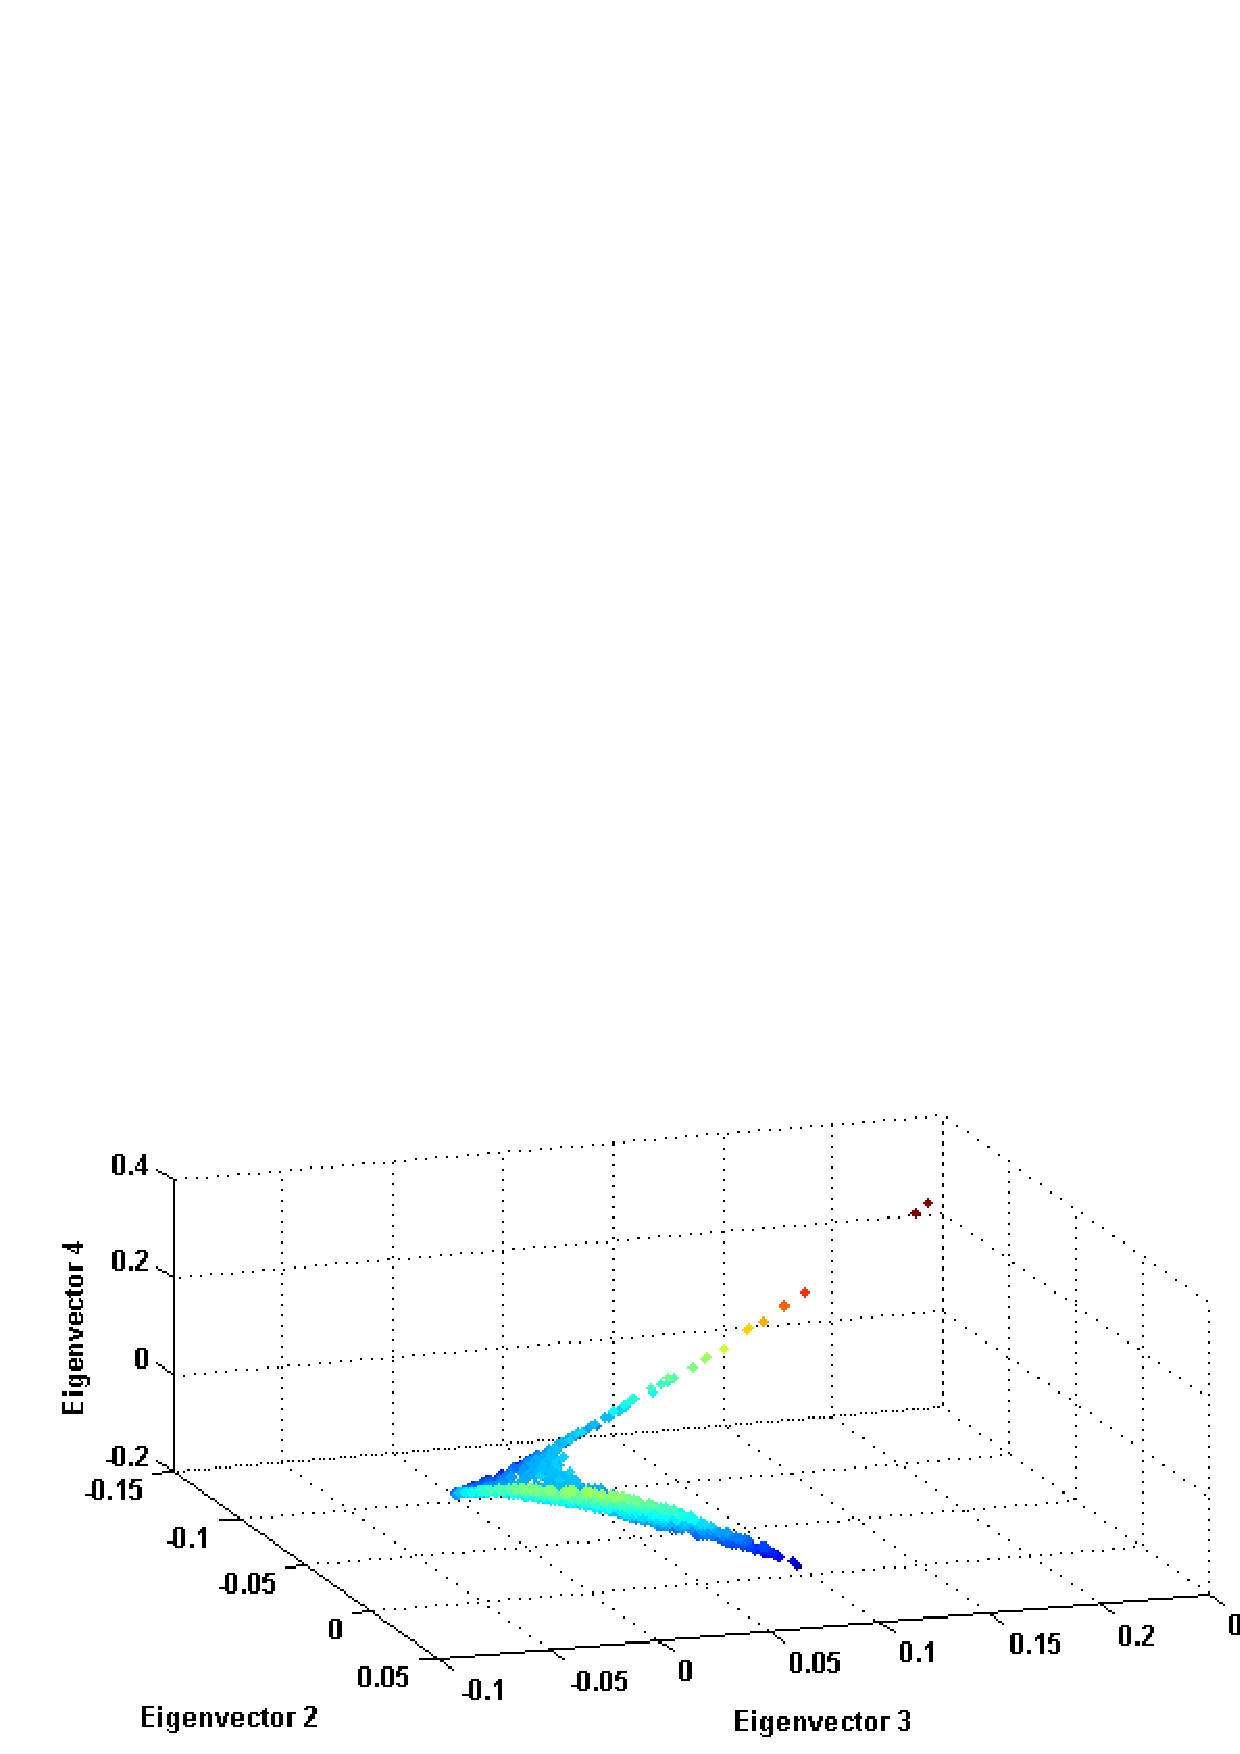
\includegraphics[width=0.81\textwidth]{CL1b.pdf}
    \caption{\label{fig:CL1b} A $3-d$ plot suggesting that the fourth
      eigenvector of the random walk matrix -calculated using the
      subgraph similarity measure- for the case of the two parameter
      family of Chung-Lu graphs can be expressed as a function of the
      second and third eigenvectors: it does not capture a new
      direction in the space of our sample graphs.  }
  \end{center}
\end{figure}


\begin{figure}
  \begin{center}
    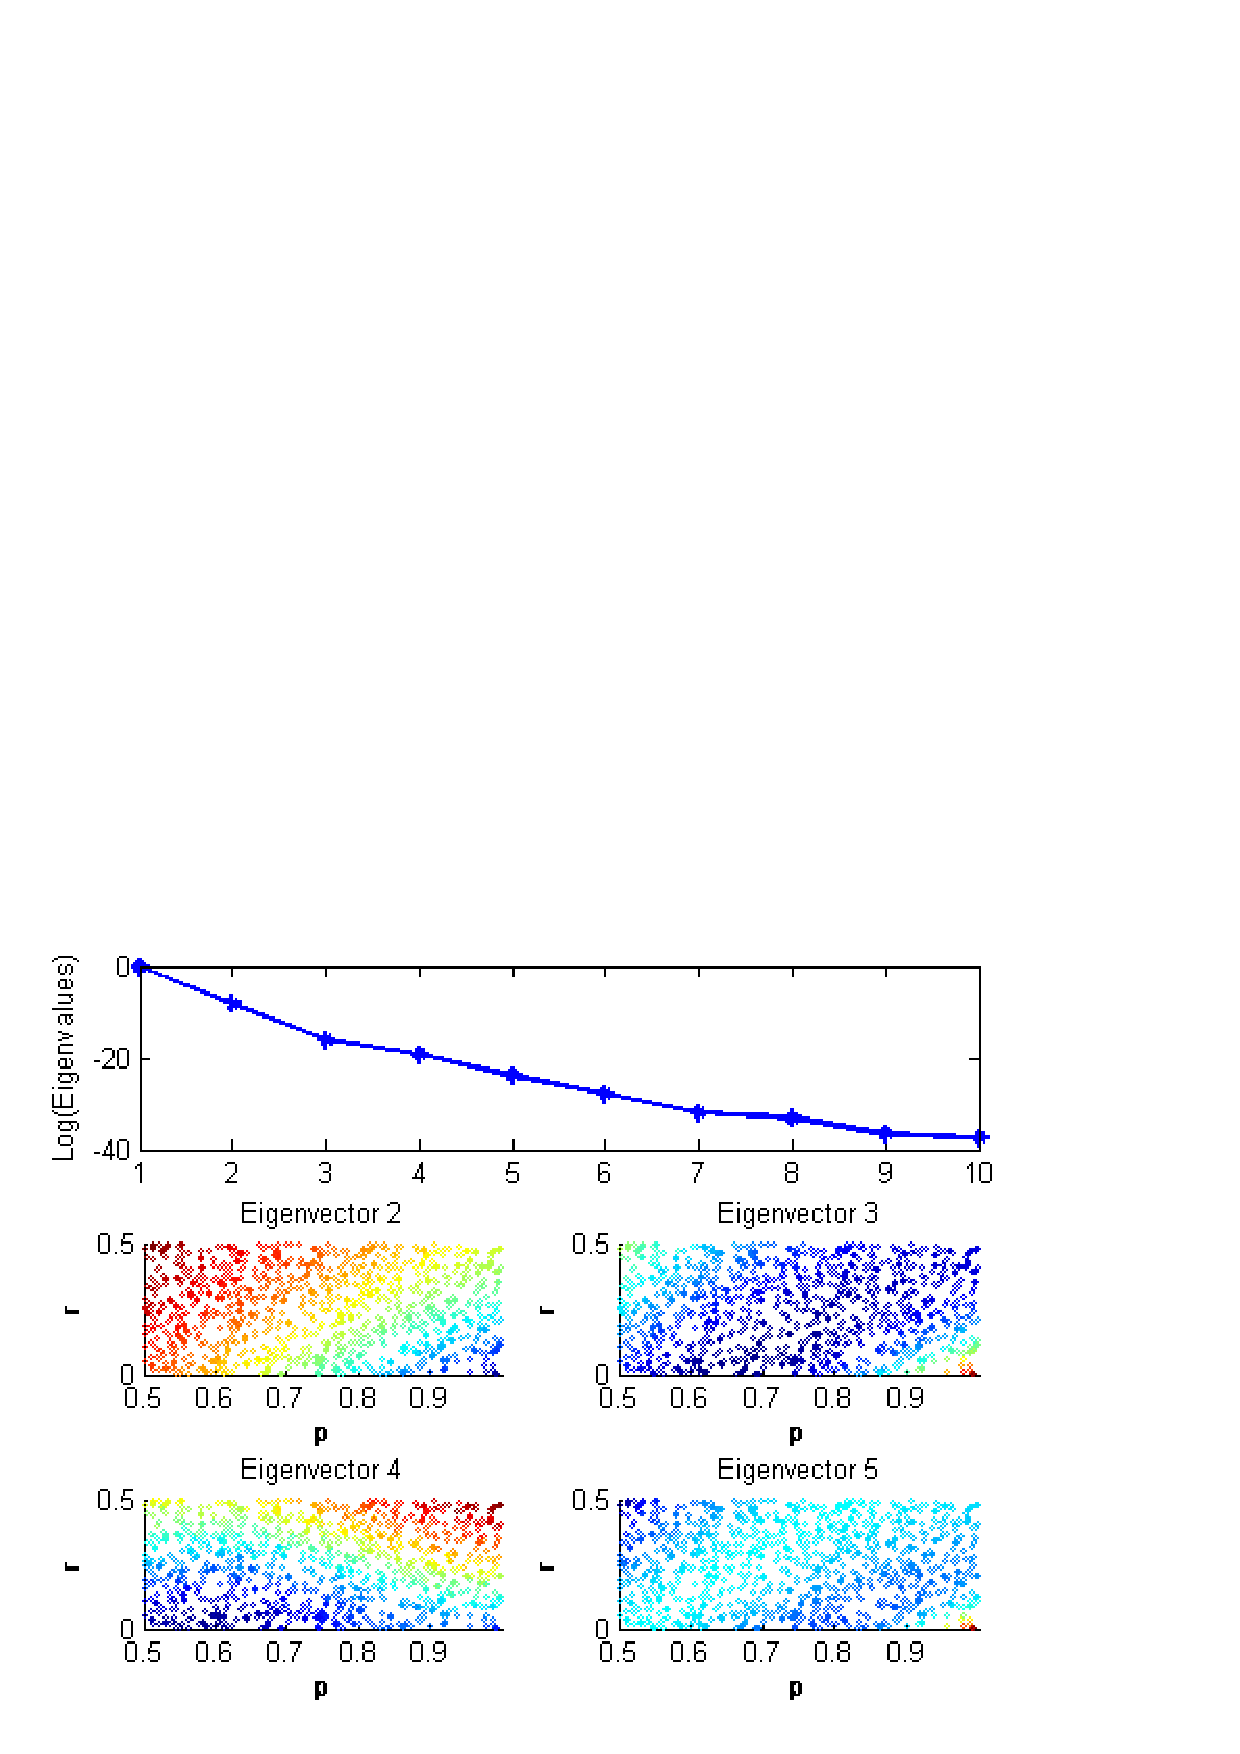
\includegraphics[width=0.81\textwidth]{CL2_ev.pdf}
    \caption{\label{fig:CL2} Data mining ensembles of two-parameter
      Chung-Lu graphs: The leading eigenvalues of the random walk
      matrix calculated using our spectral similarity measure are
      first plotted.  The corresponding first four non-trivial
      eigenvectors are then illustrated in a way that brings forth
      their relation to the construction parameters $p$ and $r$.  In
      these plots, each graph is denoted as a point.  The $x$ and $y$
      coordinates of the point correspond to the parameters $p$ and
      $r$ used to construct that particular graph.  The graphs are
      colored based on the magnitude of their components in the
      eigenvectors of the random walk matrix $A$.  }
  \end{center}
\end{figure}

\begin{figure}
  \begin{center}
    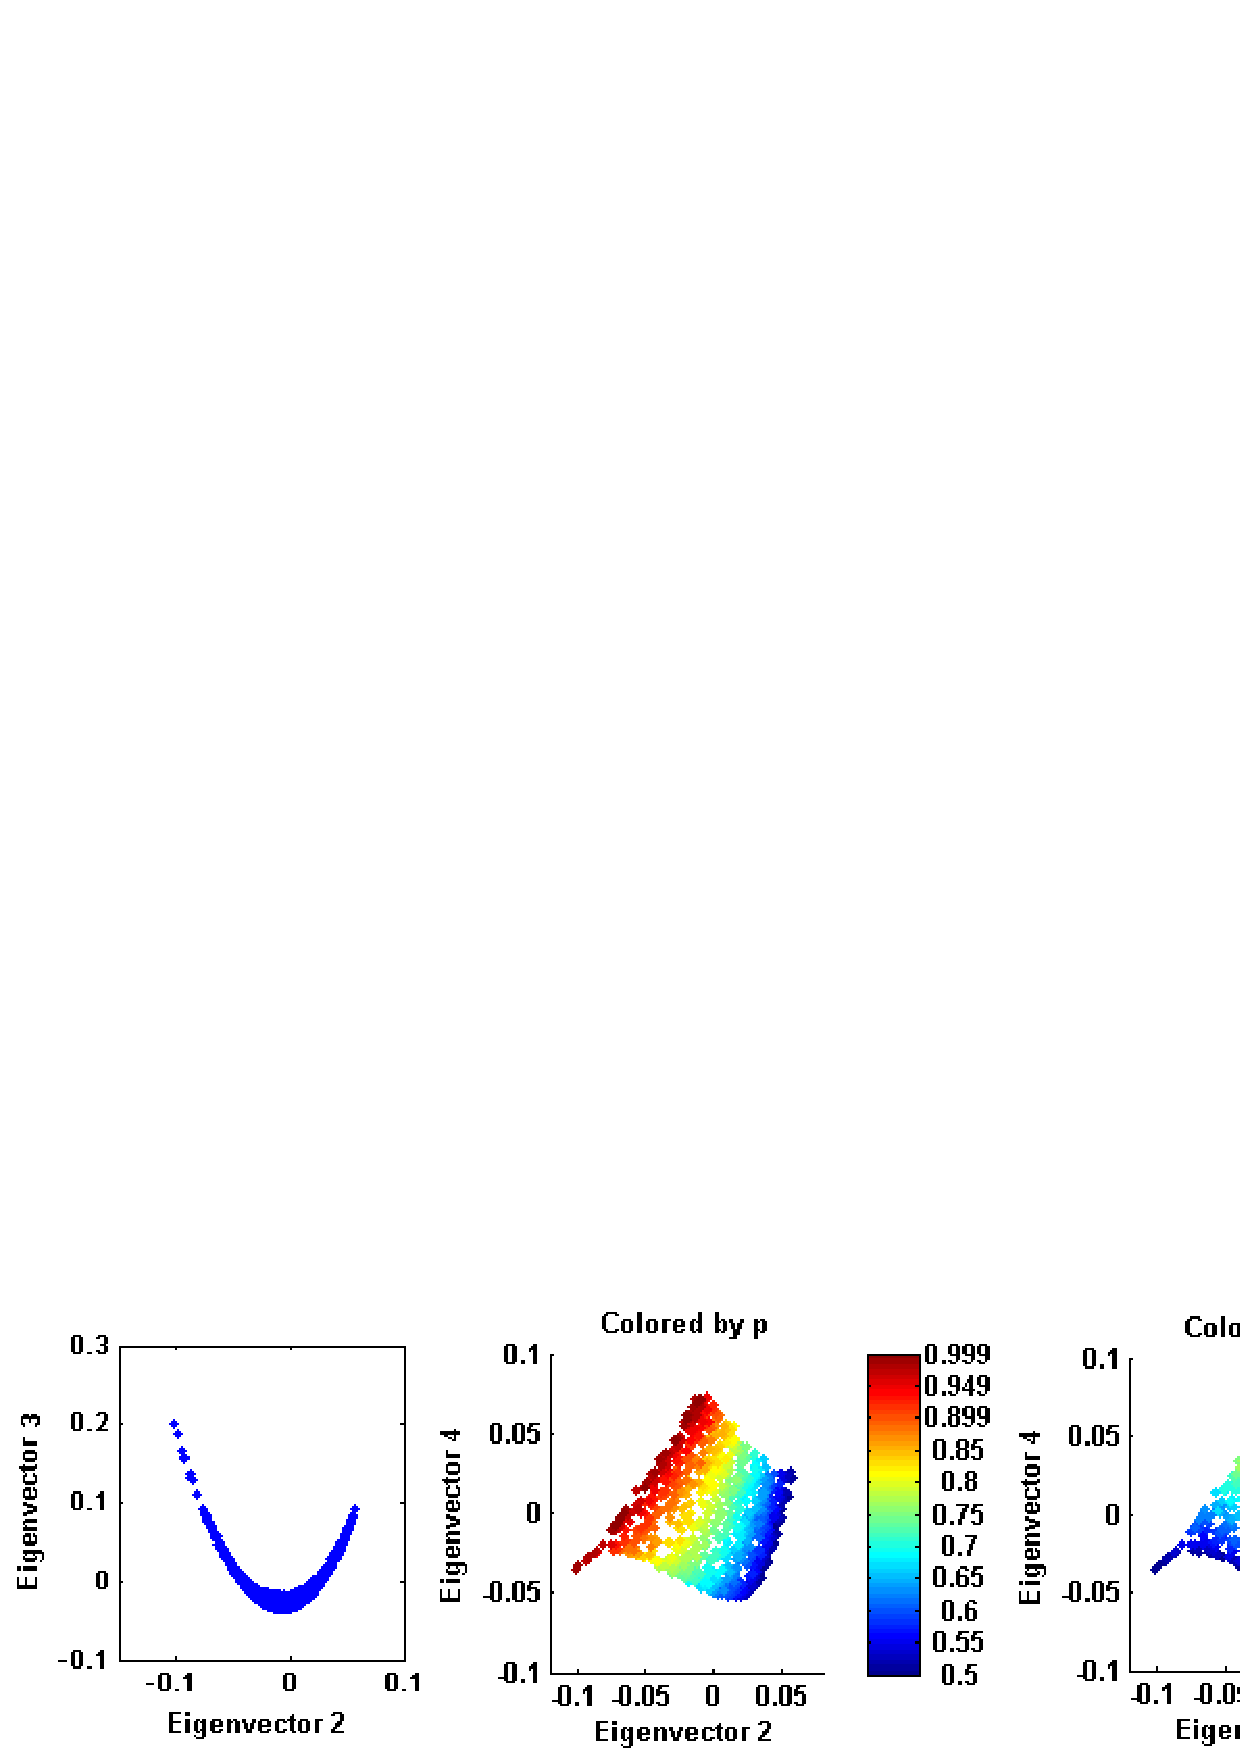
\includegraphics[width=0.81\textwidth]{CL2ab.pdf}
    \caption{\label{fig:CL2ab} Data mining the two-parameter family of Chung-Lu graphs using the subgraph similarity metric
      leads to an apparent two-dimensional
      embedding.
      % 
      In these plots the $x$ and $y$ coordinates of each point (i.e. of each graph in the dataset)
      denote the components of that particular graph in the second and third (resp., fourth) eigenvectors of the random walk matrix
      for the left plot (resp., middle and right plots).
      % 
      Each point is also colored based on the parameter values of $p$
      (middle plot) and $r$ (right plot) used to construct the
      particular graph.  }
  \end{center}
\end{figure}

We now consider a slightly richer dataset, where the graphs are
constructed using two independent parameters.
% 
The definition of this illustrative family of graphs is based on the
Chung-Lu algorithm \cite{Chun02connected}.
% 
For a graph consisting of $n$ vertices (here $n=100$), following their
original algorithm, we begin by assigning a weight $w_i$ to each
vertex $i, 1 \leq i \leq n$
% 
The weights we chose have the two-parameter form $w_i = np(i/n)^r$.
% 
The probability $P_{ij}$ of existence of the edge between vertices $i$
and $j$ is given by $P_{ij}=min(Q_{ij},1)$, where

\begin{equation}\label{}
  Q_{ij} = \frac{w_iw_j}{\sum_{k}{w_k}}.
\end{equation}

Once the edge existence probabilities are calculated, a graph can be
constructed by sampling uniform random numbers between $0$ and $1$ for
every pair of vertices $(i,j)$ and placing an edge between them if the
random number is less than $P_{ij}$.
% 
Note that in the original Chung-Lu algorithm $P_{ij}=Q_{ij}$.
% 
If the weights are chosen such that $Q_{ij} <= 1, \forall (i,j)$, then
the expected value of the degree of node $i$ would be equal to the
chosen weight values $w_i$.
% 
If any $Q_{ij}$ exceeds the value of $1$, this would no longer be the
case \cite{Chun02connected}.

% 

The model selected here has $2$ construction parameters: $p$ and $r$.
% 
If $r=0$, the resulting graphs are Erd\"{o}s-R\'{e}nyi graphs and the
parameter $p$ represents the edge density.
% 
When $p=1$ and $r=0$, the resulting graphs are complete.
% 
As $r$ is increased, this procedure creates graphs whose degree
distributions are skewed to the left (long tails towards lower
degrees).
% 
The degree distributions resulting from creating graphs with various
combinations of parameters $p$ and $r$ are shown in Fig.~\ref{fig:CL}.
% 

For our illustration, $1000$ graphs were created using this model with
$n=100$ nodes each.
% 
The values of $p$ and $r$ were chosen by uniformly sampling in the
interval $(0.5,1)$ and $(0,0.5)$ respectively.
% 
The diffusion maps algorithm was used on this set of graphs exactly as
described in the first case.
% 
As we will discuss below, the results obtained using the two
similarity measures that we consider in this paper, while conveying
essentially the same qualitative information, have visible
quantitative differences.
% 


The first $10$ eigenvalues of the random walk matrix calculated by
using the subgraph approach for evaluating similarities are shown in
the top plot of Fig.~\ref{fig:CL1}.
% 
The first four non-trivial eigenvectors are plotted below.
% 
In these plots, each of the $1000$ graphs is represented as a point in
the $p-r$ two parameter plane.
% 
The colors represent the magnitude of the components of the
corresponding graph data on each of the first $4$ non-trivial
eigenvectors.
% 
The gradient of colors in these plots suggest the direction of each of
these eigenvectors in the $p-r$ plane.
% 
However, a more careful inspection of the plots is required to
determine independent subsets of these eigenvectors. A quantitative
approach to this issue can be found in \cite{dsilva2015parsimonious}.
% 
To help explore this, we plot eigenvectors $2$ and $3$ against each
other in Fig.~\ref{fig:CL1a}.
% 
The figure clearly suggests (through its obvious two-dimensionality)
that these two eigenvectors are independent of each other.
% 
Furthermore, when the points in these plots are colored by the two
parameters $p$ and $r$ used to construct the graphs, two independent
directions - a roughly ``left-to-right" for $p$ and a roughly
``top-to-bottom" for $r$- can be discerned on the $v_2 - v_3$
manifold, Fig.~\ref{fig:CL1a}.
% 
This strongly suggests that the Jacobian of the transformation from
$(p,r)$ to $(v_2,v_3)$ is nonsingular on our data.
% 
Thus, these two eigenvectors, obtained solely through our data mining
approach, can equivalently be used to parameterize the set of graphs
constructed using the parameters $p$ and $r$.
% 
The components of the fourth eigenvector plotted in terms of these two
leading eigenvectors in Fig.~\ref{fig:CL1b} are strong evidence that
this fourth eigenvector is completely determined by (is a function of)
the second and third ones.
% 
In other words, the fourth eigenvector ``lives in the manifold"
created by the second and third eigenvectors, and hence does not
convey more information about (does not span new directions in) our
graph dataset.


We now focus on similar results obtained with the same dataset, but
now using our spectral approach for measuring similarity.
% 
The eigenvalues and eigenvectors of the random walk matrix obtained by
this approach are reported in Fig.~\ref{fig:CL2}.
% 
As before, we plot the leading eigenvectors against each other in
Fig.~\ref{fig:CL2ab}.
% 
The plot of eigenvector $2$ versus eigenvector $3$ appears as a smooth
``almost" curve, suggesting a strong correlation, while the plot of
eigenvector $3$ versus eigenvector $4$ clearly shows
two-dimensionality.
% 
These figures suggest that eigenvectors $2$ and $3$ parameterize the
same direction in the $p-r$ plane, while eigenvector $4$ parameterizes
a second, new direction in this plane.
% 
Hence, eigenvectors $2$ and $4$ constitute independent dimensions in
the space of our sample graphs.
% 

Once again, we have recovered (through data mining) two independent
directions in our sample family of graphs that were constructed using
two independent parameters.
% 
Although the results obtained using the subgraph and the spectral
approaches in this case are quantitatively different in their details,
they are both successful in recovering two independent coordinates in
the space of graphs given as input to the data mining algorithm.
% 
The $2D$ manifold resulting from the subgraph approach seems visually
better at visually capturing the behavior of the original $p-r$ plane.
% 
The ``quality" of these parametrizations will clearly be affected by
the details used in the data-mining procedure and, in particular,
those affecting the similarity measure evaluation: the number of
subgraph densities kept, the choices for numerical constants such as
$\lambda$ in the subgraph approach, $\epsilon$ in diffusion maps, etc.
% 
An obvious criterion in the selection of these method parameters is to
make the Jacobian of the transformation from the ``natural" to the
``data-mining-based" parametrizations as far from singular as
possible.


\subsection{\label{ss:dm} Test case $3$: Graphs from a dynamic graph
  evolution model}

In the two examples given above, the graphs in each dataset were
created using prescribed rules of a model controlled by one or more
parameters.
% 
Let us now consider a case where the graph dataset comes from sampling
graphs from a dynamical process at regular time intervals.
% 
The dynamical process could either be an empirically evolving graph
system or a dynamic model with prescribed rules of evolution.
% 
We consider the latter case for illustration, making use of a simple
model of a random evolution of networks \cite{bold2014equation}.
% 
A brief description of the model is given here.
% 
Starting from an initial graph, the model rules update the graph
structure at every time step by repeatedly applying the following
operations:

\begin{enumerate}
\item A pair of nodes selected at random are connected by an edge if
  they are not already connected to each other.
\item An edge chosen uniformly at random is removed with probability
  $r=0.1$.
\end{enumerate}

% 
The details of the model behavior are discussed in
\cite{bold2014equation}.
% 
Here, we will focus only on the characteristics of the model evolution
necessary to explain the results of data mining.
% 
For this particular graphical model, it is known that the degree
distribution functional $d: (G,t) \rightarrow \mathbb{N}$ evolves
smoothly in time as shown in the left plot of Fig.~\ref{fig:K_d3}.
% 
Furthermore, it is also known that the evolution of degrees is
decoupled from (and slower than) the evolution of all higher order
properties such as triangles, degree-degree correlations, and so on.
% 
Thus the information about the dynamic evolution of the graphs
according to this model can be sufficiently captured by studying the
degrees.
% 
A principal component analysis of sequences of degrees starting from
different initial conditions was performed, and the two leading
principal components are also plotted in Fig.~\ref{fig:K_d3}.
% 
The first principal component (PCA), labeled PC $1$, corresponds the
steady state degree distribution while the second principal component
PC $2$ corresponds to the direction along which the degree
distribution decays the slowest towards steady state.
% 
Since the degree distribution is known to be the most significant
variable in this model, PC $1$ and PC $2$ are good variables to track
the evolution of the graphs over time.
% 
In fact, as shown in \cite{bold2014equation}, one can write explicit
Fokker-Planck equations for the evolution of the distribution of
(appropriately shifted and scaled) degrees.
% 
The eigenfunctions of the corresponding eigenvalue problem are Hermite
polynomials, the first two of which have the qualitative forms,
$\exp(-x^2)$ and $x \cdot \exp(-x^2)$, which are expressed in PC $1$
and PC $2$ respectively.
% 


Let us now ignore our knowledge of the dynamical process and only
consider the data: the graph sequences created by the process.
% 
Our goal is to use diffusion maps to find out good variables to
characterize these graphs.
% 
Since the graph data used for data mining come from a dynamical
process, the variables obtained through data mining should correspond
to the dynamics of the process.
% 
In other words, we expect the data mining variables and the variables
PC $1$ and PC $2$ to convey similar information about the graphs.
% 
As before, we will use both the subgraph and spectral similarity
measures to get the results.
% 
The eigenvalues and the first two non-trivial eigenvectors of the
random walk matrix in diffusion maps are shown for both the subgraph
and spectral similarity measures in Figs.~\ref{fig:K1} and
\ref{fig:K2} respectively.
% 
The plots are shown such that the points (corresponding to the graphs)
are plotted in the plane of the principal components PC $1$ and PC $2$
and are colored by the eigenvectors for comparison.
% 
In both cases, the results show that the second and third eigenvectors
have the most variation (as indicated by the gradient of colors) in
the directions of PC $2$ and PC $1$ respectively.
% 
Conversely, we can plot the graphs in terms of the diffusion map
eigenvectors (the new embedding) and color them based on PC $1$ and PC
$2$ as shown in Figs.~\ref{fig:K1a} and \ref{fig:K2a} corresponding to
the subgraph and spectral similarity measures respectively.
% 
This indicates that the first two non-trivial eigenvectors are roughly
one-to-one with PC $2$ and PC $1$ respectively.

For a quantitative verification of this observation, we can consider
the mapping $f : \boldsymbol{\phi} \rightarrow \boldsymbol{p}$ between
the diffusion map eigenvectors $ \boldsymbol{\phi} = (\phi_2, \phi_3)$
and the two principal components $\boldsymbol{p} = (p_1, p_2)$. By
suitably discretizing the space of graph snapshots, we can directly
compute the average rate of change of each principal component with
respect to each eigenvector coordinate. This is achieved by
considering all graphs in a specific neighborhood of the diffusion map
space and averaging the rate of change of $p_{\{1,2\}}$ with respect
to each of $\phi_1$ and $\phi_2$ within that neighborhood, thus
providing a local estimate of each partial derivative
$\partial_{\phi_j} p_i $. As outlined in Fig. \ref{fig:J}, this allows
us to verify that the Jacobian of $f$ is non-zero everywhere, giving
further evidence that the transformation between the two is bounded
away from zero.

To summarize, we have shown an illustrative example here in which
graphs collected from a dynamic process were used to recover important
variables parametrizing the evolution of the process.
% 
We considered a simple example for which theoretical results were
available, so that we were able to compare the results from data
mining with those from theory.
% 
In problems where such theoretical results are not available, one can
use data mining to gain an understanding about the primary driving
factors in the dynamics of the system.
% 


\begin{figure}
  \begin{center}
    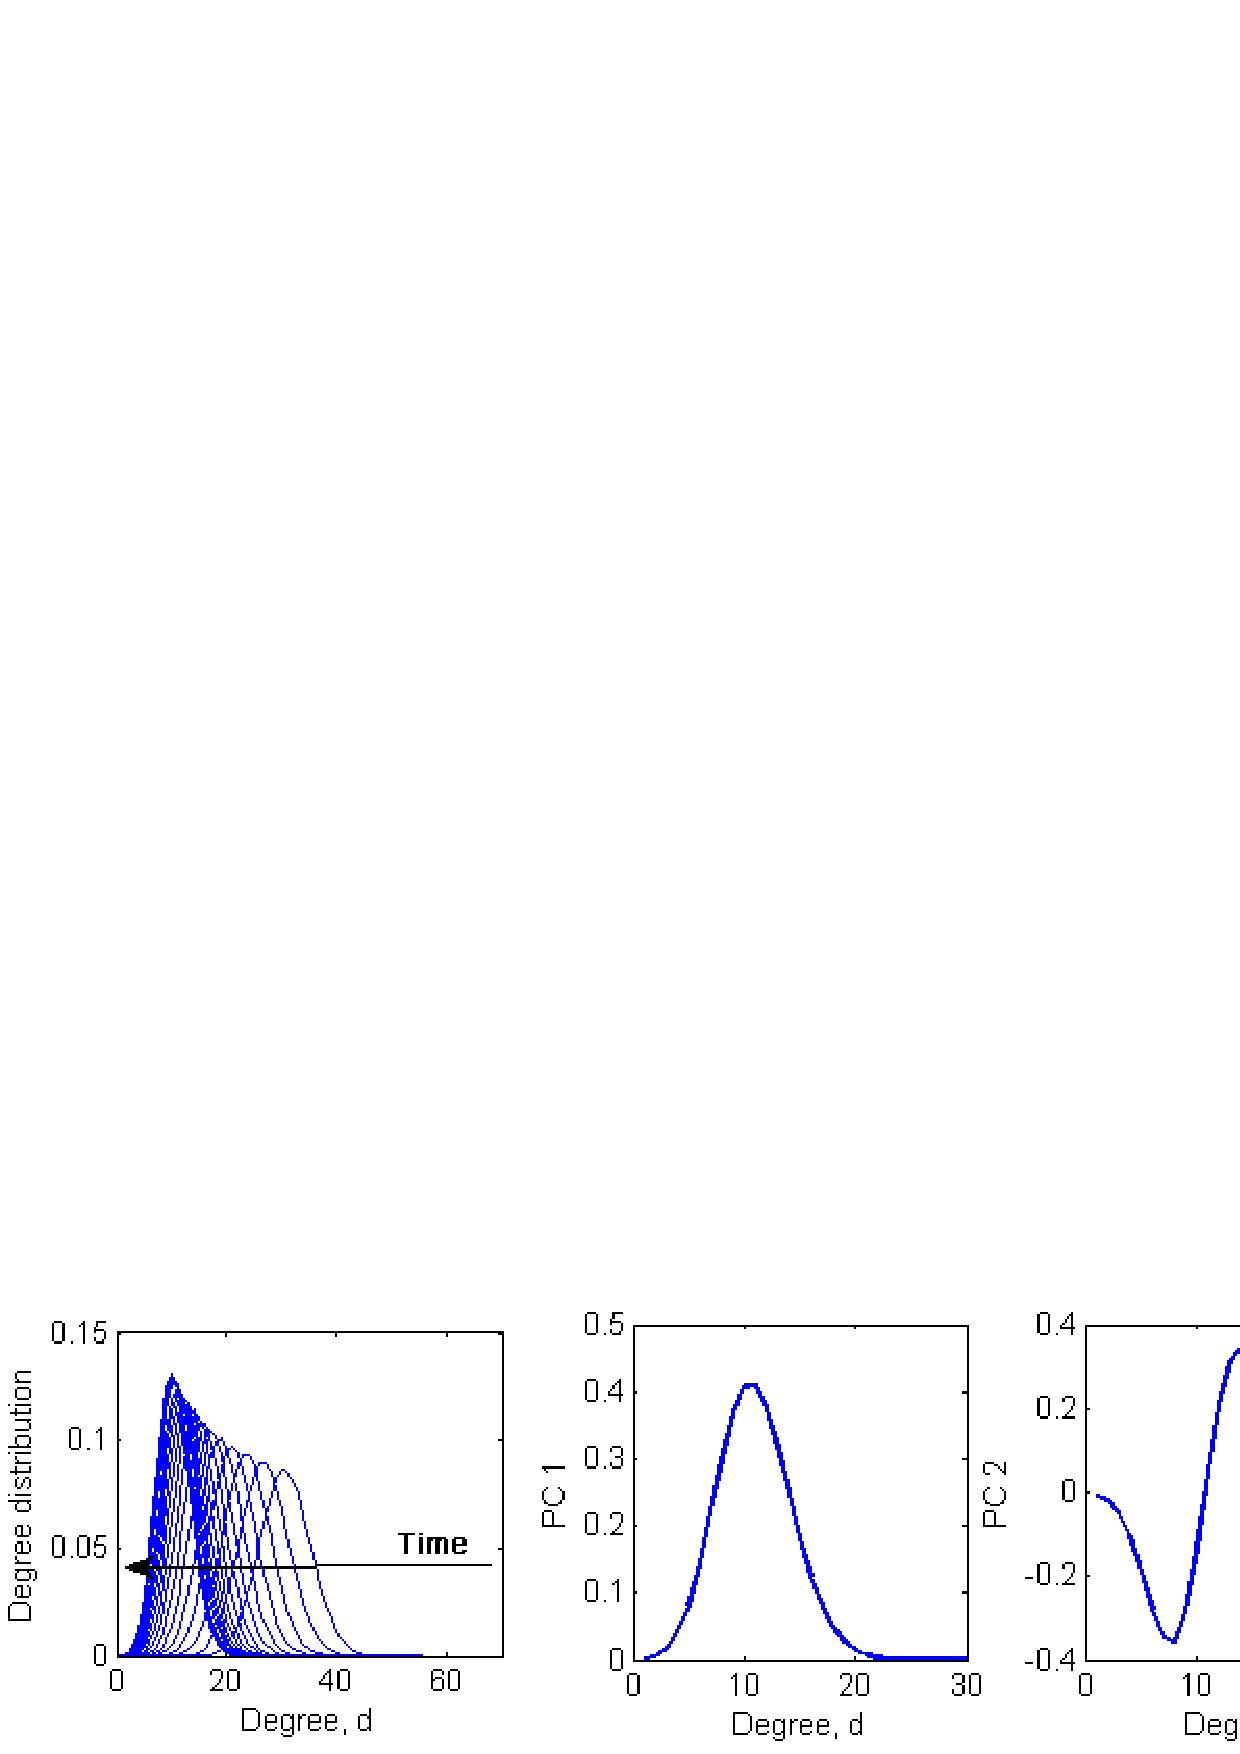
\includegraphics[width=0.81\textwidth]{K_d3.pdf}
    \caption{\label{fig:K_d3} The evolution of degree distribution
      over time from a single initial condition is shown on the left;
      The first two principal components (obtained through PCA) of
      sequences of degree distribution starting from different initial
      conditions is shown on the right.  }
  \end{center}
\end{figure}

\begin{figure}
  \begin{center}
    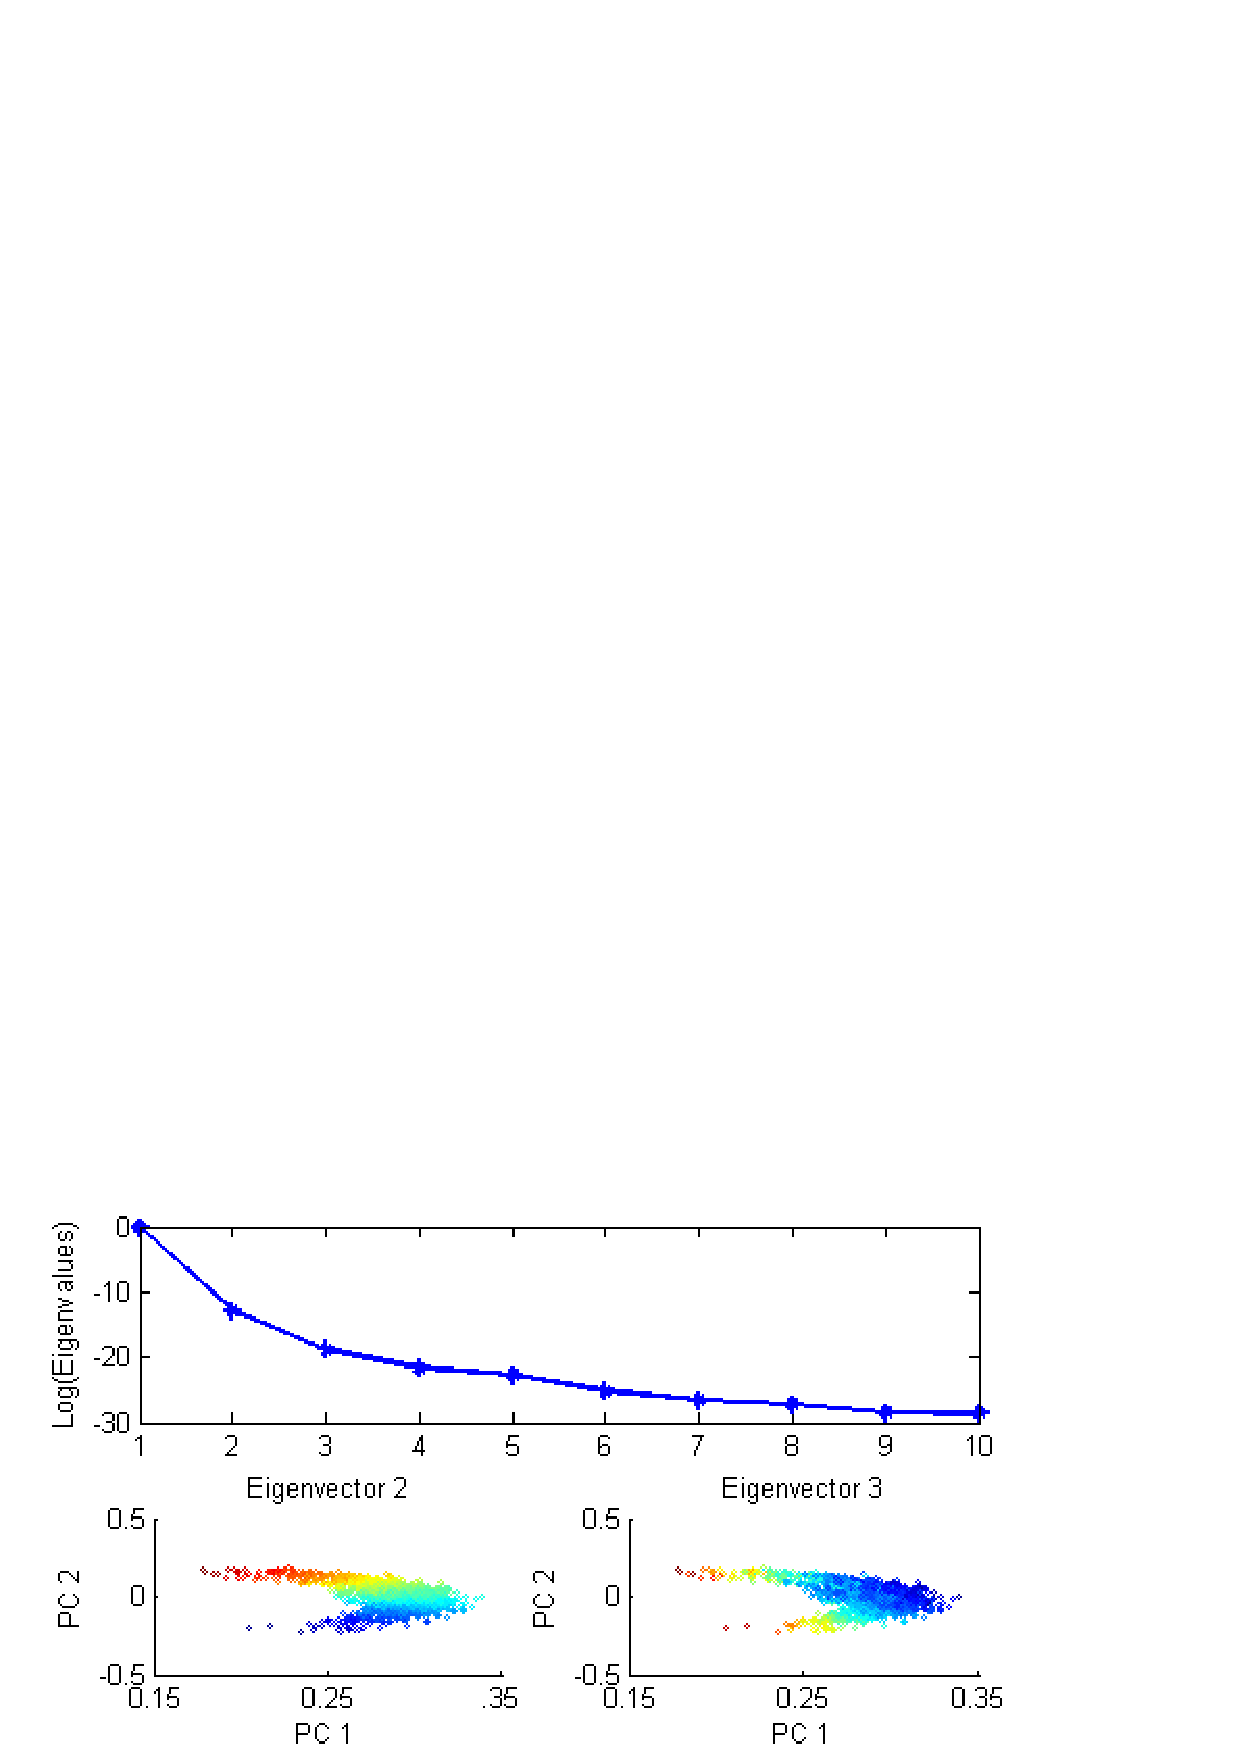
\includegraphics[width=0.81\textwidth]{K1_ev.pdf}
    \caption{\label{fig:K1} Data mining results for graphs collected
      from the dynamic graph evolution model: The principal
      eigenvalues of the random walk matrix calculated using the
      subgraph similarity measure are plotted.  The corresponding
      first four non-trivial eigenvectors are shown here. In these
      plots, each graph is denoted as a point.  The $x$ and $y$
      coordinates of the point correspond to the parameters PC $1$ and
      PC $2$ described in the text.  The graphs are colored based on
      the magnitude of the eigenvectors of the random walk matrix $A$.
    }
  \end{center}
\end{figure}

\begin{figure}
  \begin{center}
    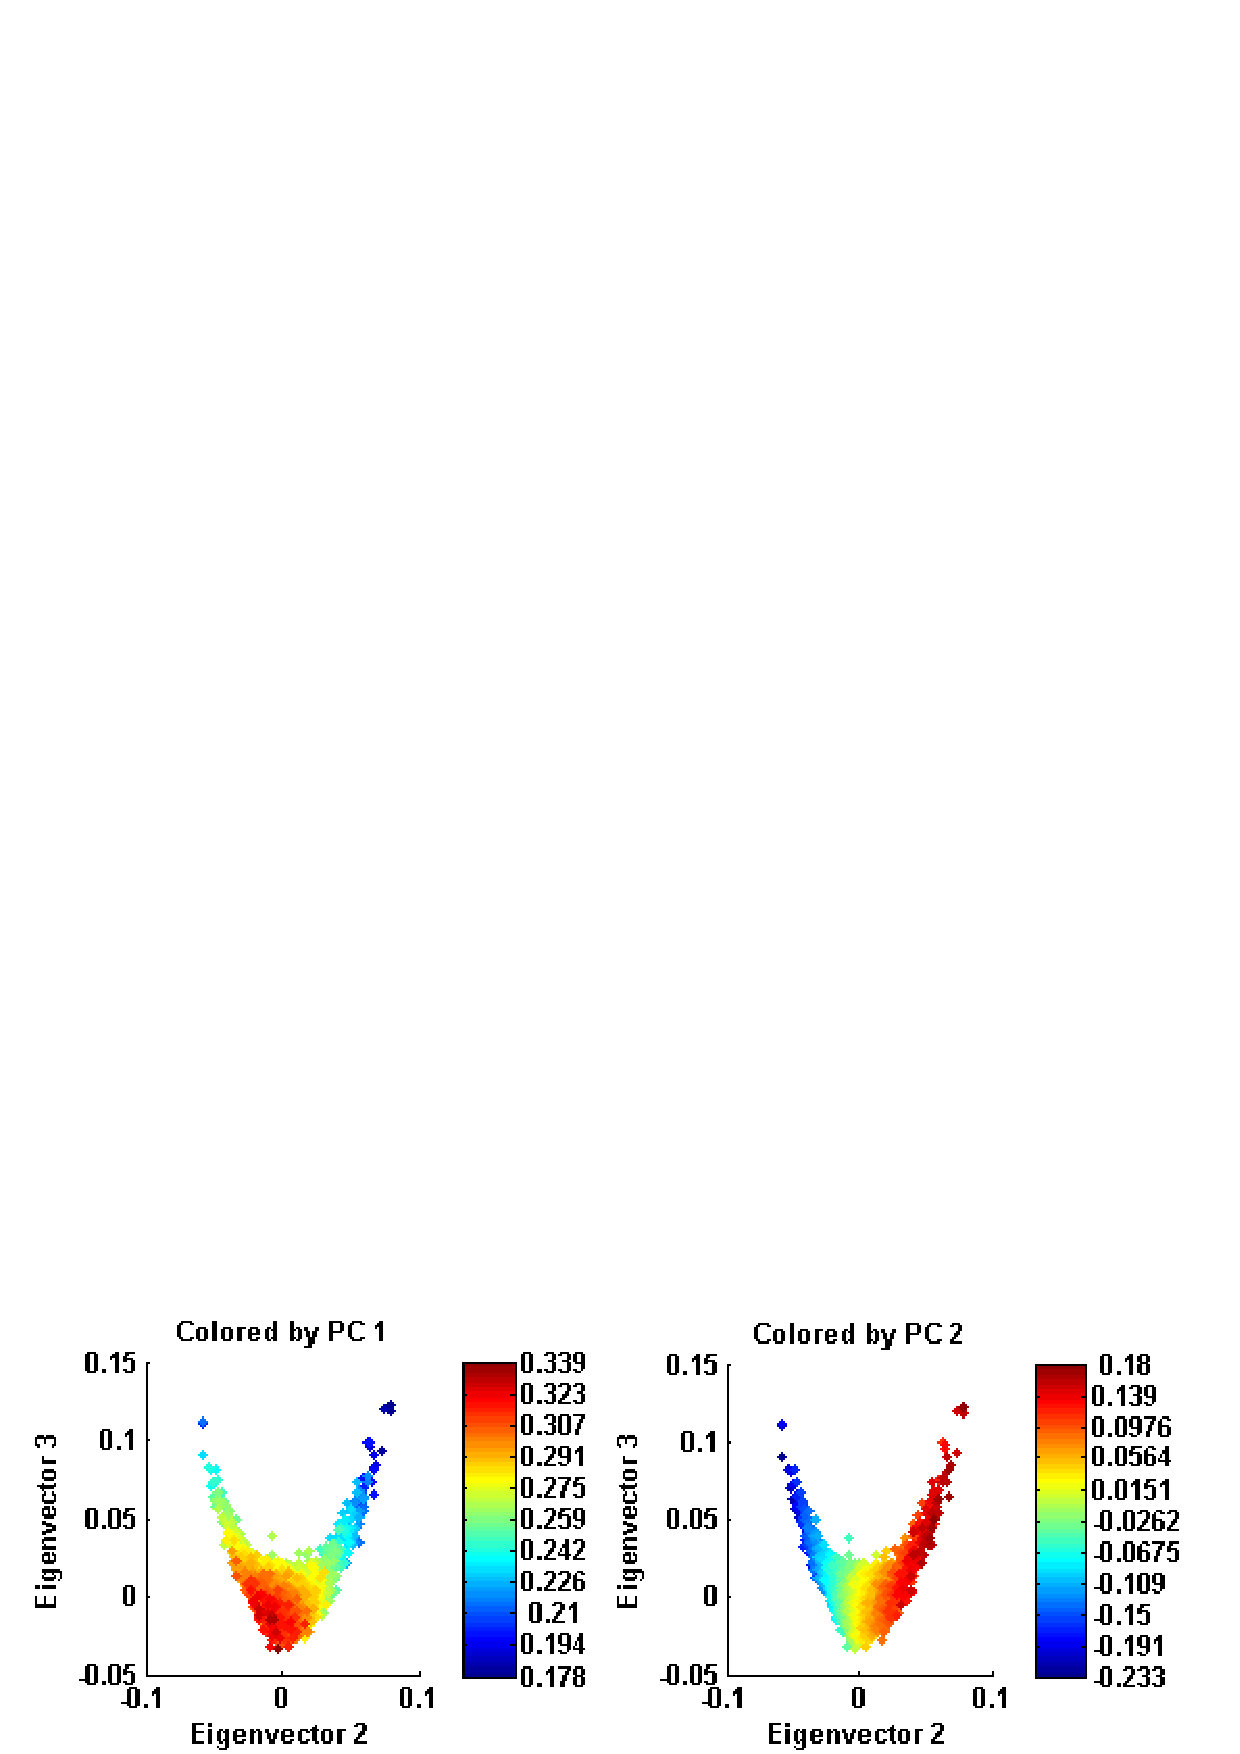
\includegraphics[width=0.81\textwidth]{K1a.pdf}
    \caption{\label{fig:K1a} The graphs collected from the dynamic
      model are plotted in terms of the two eigenvectors shown in
      Fig.~\ref{fig:K1}. The points corresponding to the different
      graphs are colored based on the first two principal components
      of the degree distribution corresponding to these graphs.  }
  \end{center}
\end{figure}

\begin{figure}
  \begin{center}
    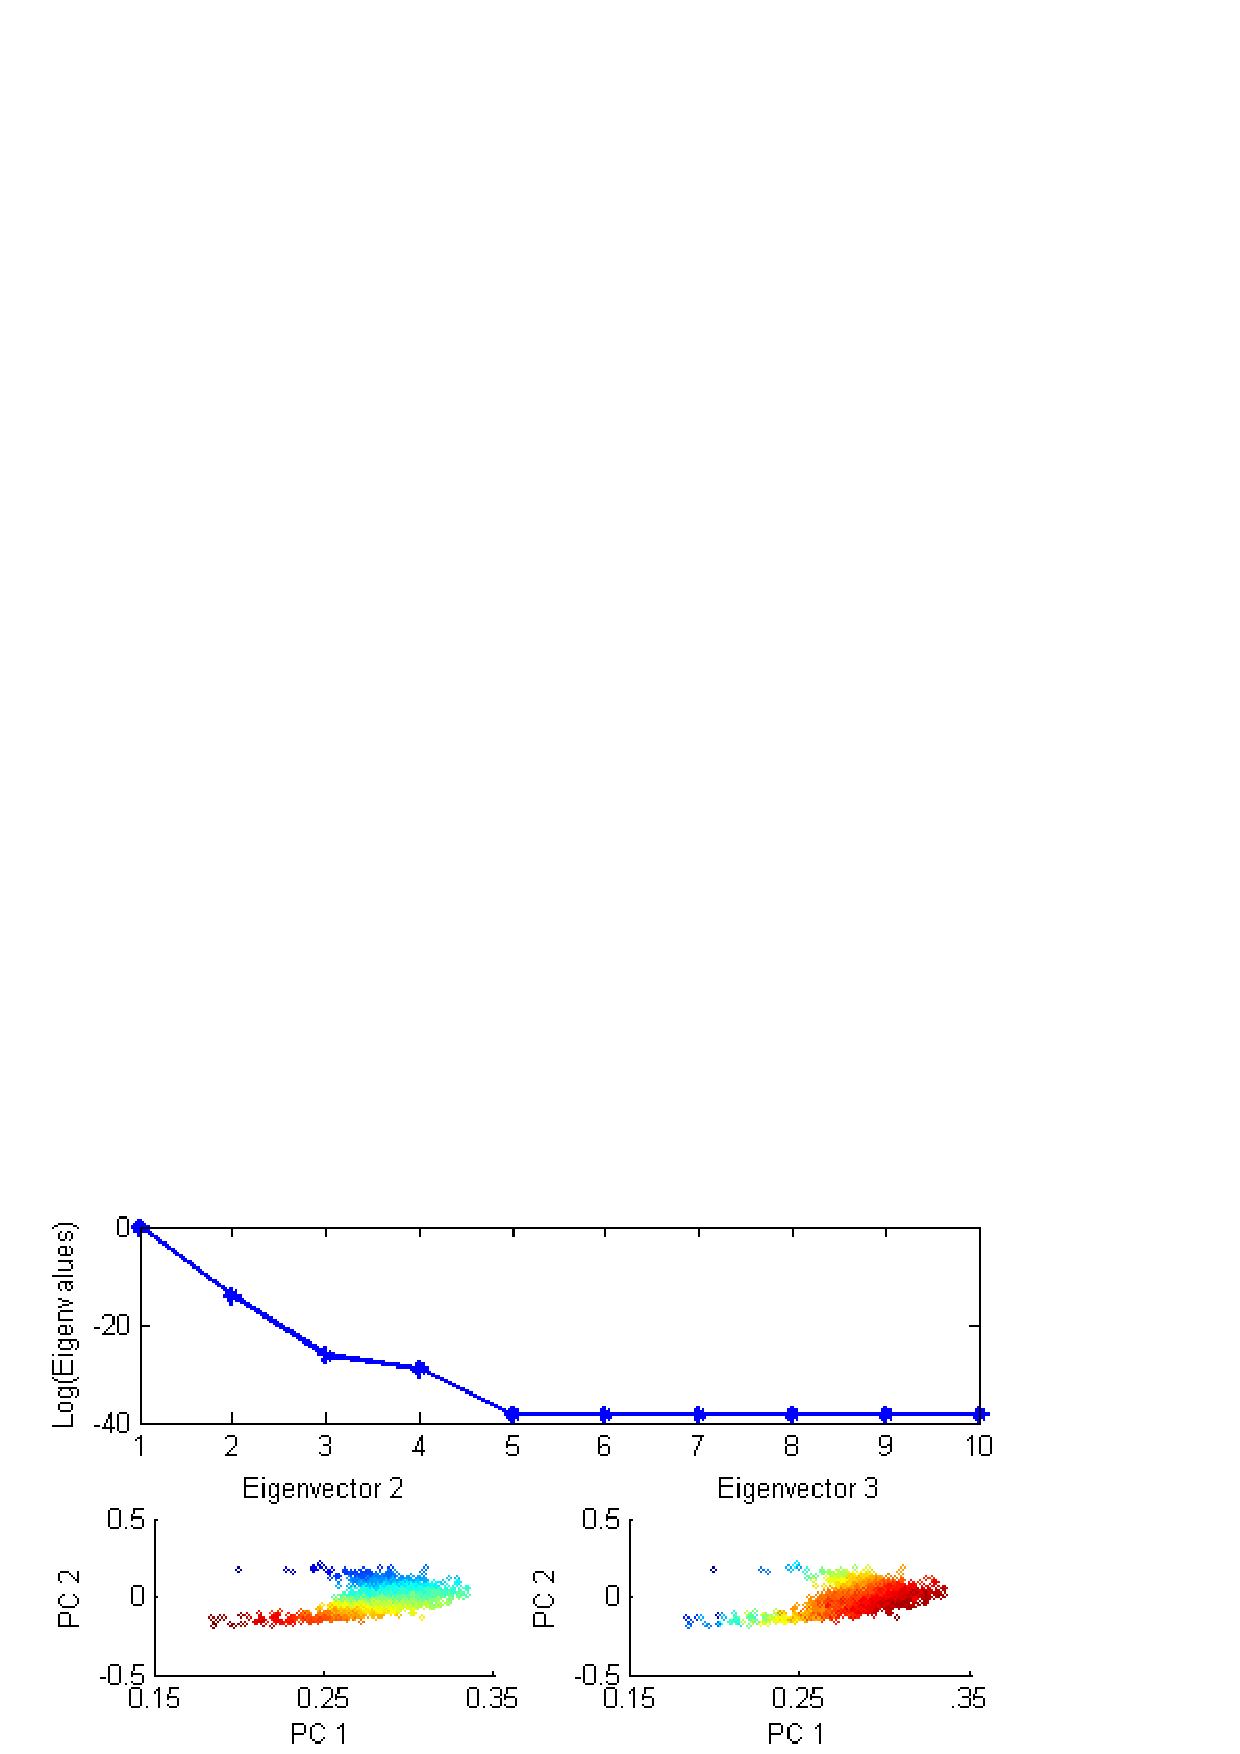
\includegraphics[width=0.81\textwidth]{K2_ev.pdf}
    \caption{\label{fig:K2} Data mining results for graphs collected
      from the dynamic graph evolution model: The principal
      eigenvalues of the random walk matrix calculated using the
      spectral similarity measure are plotted.  The corresponding
      first four non-trivial eigenvectors are shown here. In these
      plots, each graph is denoted as a point.  The $x$ and $y$
      coordinates of the point correspond to the parameters PC $1$ and
      PC $2$ described in the text.  The graphs are colored based on
      the magnitude of the eigenvectors of the random walk matrix $A$.
    }
  \end{center}
\end{figure}


\begin{figure}
  \begin{center}
    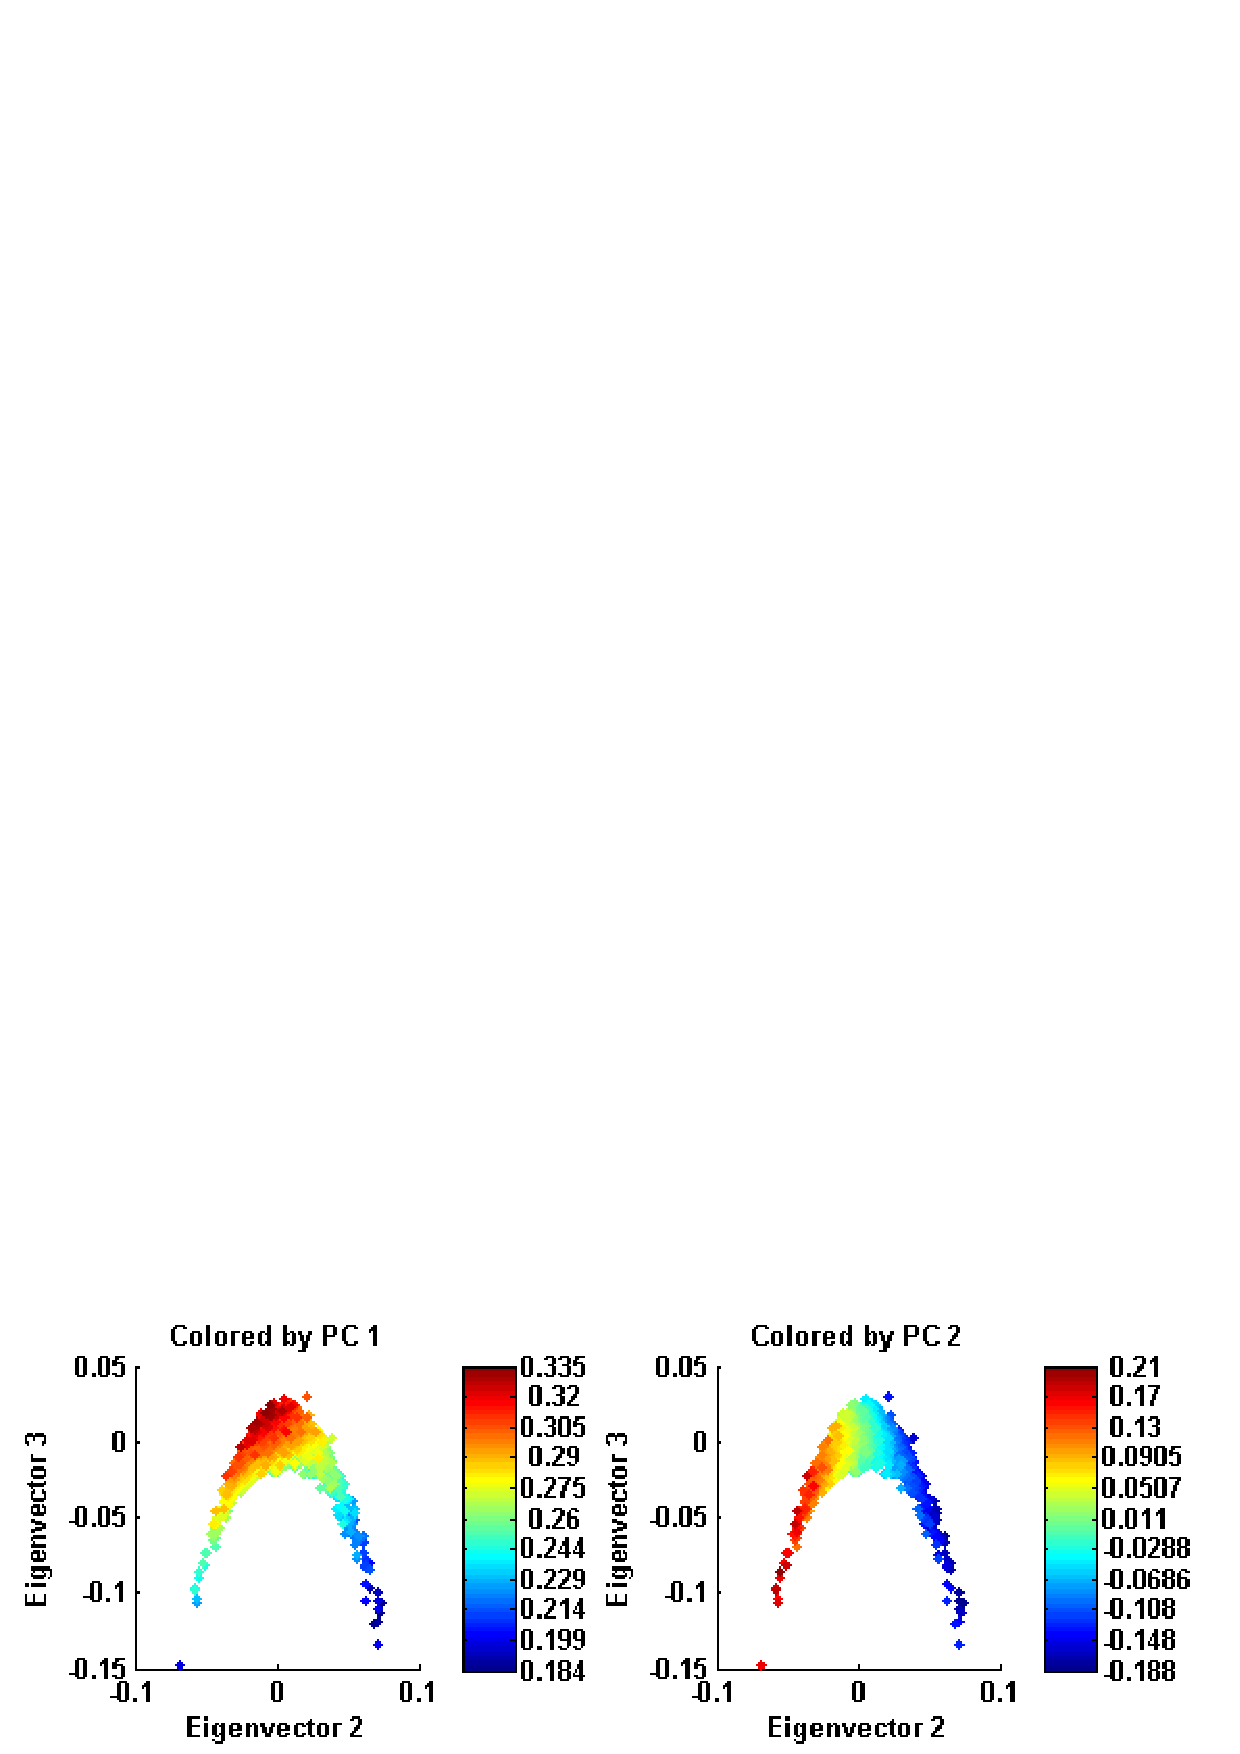
\includegraphics[width=0.81\textwidth]{K2a.pdf}
    \caption{\label{fig:K2a} The graphs collected from the dynamic
      model are plotted in terms of the two eigenvectors shown in
      Fig.~\ref{fig:K2}. The points corresponding to the different
      graphs are colored based on the first two principal components
      of the degree distribution corresponding to these graphs.  }
  \end{center}
\end{figure}

\begin{figure}
  \begin{center}
    \includegraphics[width=1\textwidth]{alljcb.pdf}
    \caption{\label{fig:J} Data mining results for graphs collected
      from the dynamic graph evolution model for a large dataset are
      shown above, colored by PC $1$ and PC $2$ respectively. The two
      eigenvectors deemed significant here were the second and fourth,
      with the same DMAP procedure performed as before. Below, each
      graph datum is colored by the individual partial derivatives on
      the left and by the Jacobian on the right. We easily notice that
      $\partial_{\phi_1} p_2$ remains positive everywhere, as was
      expected, while the Jacobian does not change sign - indicating
      that the transformation is one-to-one.  }
  \end{center}
\end{figure}


\section{\label{sec: ef} Equation-Free Methods for Accelerating Graph
  Evolution Computations}


By extracting the important variables governing the evolution of a
graph-based dynamical process, we can investigate the mapping between
these variables and temporal instances of the process. To do so, we
turn our attention to Equation-Free (EF) modeling methods
\cite{kevrekidis2003equation} \cite{kevrekidis2004equation} and their
applications to network-based dynamical systems. EF methods provide a
framework for working with low-dimensional representations (``coarse
variables") of a dynamical system, even where closed form expressions
of these variables are not available. More specifically, we proceed in
two steps: firstly, a `coarse-graining' technique is used to extract a
meaningful parametrization of the dynamics of the process in question,
i.e. one encompassing all of its degrees of freedom in a lower
dimensional representation. If such a low-dimensional characterization
of the system exists, then this step identifies both its inherent
dimensionality and the suitable coarse variables that span it. Here,
we use the variables recovered by our data-mining approach as the
required coarse variables that parametrize it. The second step
involves the investigation of mappings between these coarse variables
and instances of the dynamical process. We are thus required to
construct suitable mapping operations between the coarse variables
identified in the previous step and instances of the dynamical process
in an efficient fashion. This is discussed in more detail below.



\subsection{Lifting \& Restriction}

The two key ingredients for the use of EF techniques are the
capability to move from instances of the `fine-grained' system (in
this case realizations of the evolving network) to the
`coarse-grained' representation of the system and vice-versa. We
denote the operators defining the movement between these two regimes
as {\em restriction} and {\em lifting} respectively, with the latter
usually posing a much larger computational challenge and involving
multiple instances of the former. More specifically, if we denote by
$\psi_t$ the fine-grained temporal evolution operator of the dynamical
process, we can define the coarse-grained evolution operator $\Psi_t$
as follows:
\begin{equation}
  \Psi_t ( \cdot ) = R \circ \psi_t \circ L ( \cdot ),
\end{equation}
\noindent where $R(\cdot)$ and $L(\cdot)$ denote the restriction and
lifting operations respectively.

The main idea underpinning this method is that, given a suitable
coarse description of the system and efficient lifting/restriction
operators, we do not have to work exclusively in the fine-grained
regime (i.e. by executing repeated long-term system simulations),
which is usually computationally expensive. Instead, we can restrict
to the coarse variables, advance the system in this regime (usually
using numerical estimation techniques), and then lift back to an
instantiation of the fine-grained system that is suitably close to
where direct simulation would have advanced the process. Indeed, with
the help of these operators, appropriately initialized instances of
the dynamical system are run for short bursts of time, providing local
information that can then be used to expedite analysis of the system's
dynamics. This technique can be used alongside implicit methods
\cite{marschler2014implicit} to construct an estimator that converges
to the true dynamics of the system on the slow manifold, something
that would increase the accuracy of our algorithm.


\subsection{Coarse-Projective Integration}

Various methods for the implementation of EF techniques in
network-based dynamical systems have been explored
\cite{bold2014equation} \cite{holiday2016equation}, but they usually
require an intimate understanding of the dynamical system in question
in order to implement the coarse-graining step. As mentioned
previously, here we will use the data mining procedure from
Section~\ref{sec:dm} to coarse-grain the dynamical process, without
making any explicit assumptions about its dynamics. This has the
advantage of requiring no previous information about the system in
question, and thus can be applied in a very general context. We
illustrate the confluence of the proposed data mining technique with
EF methods by demonstrating its application to Coarse-Projective
Integration (CPI) \cite{gear2003projective}, an EF technique whose
primary goal is the acceleration of the dynamical system's time
evolution by projectively integrating the coarse variables forward in
time. In a comparative analysis, we demonstrate that the temporal
evolution of the underlying dynamical system can be accelerated
through CPI.

To illustrate this, we work with the dynamical network example from
the previous section and compare our results of both a long-term
fine-grained simulation and the CPI simulation. We furthermore look at
the underlying variables, which are known to define long-term dynamics
of these two simulations, at different timesteps. This allows us to
further validate our approach. In the context of EF computations, we
use the two leading eigenvectors $(\phi_2, \phi_3)$ as the
coarse-graining variables of interest, which are obtained through our
data-mining procedure. More specifically, we begin by generating a
large (with $\sim 10^3$ datapoints) `reference' graph dataset that
contains snapshots of networks approaching the system steady state
from many directions. This is done by taking temporal snapshots of
many Erd\"{o}s-R\'{e}nyi random graphs evolving according to the
network rules, exactly as in the preceding section, and performing
DMAPs on the ensemble to get the eigenvector coordinates of each graph
datum. We define this `reference' collection of graphs as
$\{ G^i_R \}_{i = 1}^M$ and denote the diffusion variables of some
graph $G_i$ in the reference dataset by
$\phi_{ref}(G_i) = (\phi_2^i, \phi_3^i)$. It should be noted that
throughout the simulation, we will always have access to both the
network instances and corresponding eigenvectors of this precomputed
dataset. Finally, it should be noted that we are going to be working
not with individual graphs, but rather with {\em ensembles} of $N$
graphs in both transformations. We now define the exact lifting and
restriction operators.

\subsubsection{Lifting}

Our lifting operator is a mapping
$L: \mathbb{R}^2 \rightarrow \{(c_i,G_i)\}^N_{i = 1}$, from one
diffusion coordinate $\phi_0 = (\phi^0_2, \phi^0_3) \in \mathbb{R}^2$
to an ensemble of $N$ different graph-coordinate pairs, where
$c_i \in \mathbb{R}$ the coefficient associated with graph $G_i$. We
pick the ensemble of $N$ graphs from the reference dataset by looking
at graphs whose diffusion coordinates are closest to
$(\phi_2^0, \phi_3^0)$, i.e. the $N$ nearest neighbors by diffusion
distance. To compute the corresponding coefficients $c_i$, we solve
the following interpolation problem:

\begin{equation}
  \label{eq:intra}
  \phi_0 = \sum_{i = 1}^N c_i \cdot \phi_{ref}(G_i),
\end{equation}
which can be easily achieved through Singular Value Decomposition
(SVD) techniques, since we choose $N > 2$. Note that the coefficients
assigned to each graph denote the graph's `weight' in characterizing
$\phi_0$ based on its own diffusion coordinates. In short, the lifting
operator proceeds as follows:
\begin{enumerate}
\item On input $\phi_0$, find the $N$ reference graphs
  $\{G_i\}^N_{i = 1}$ whose diffusion coordinates
  $\{\phi_{ref}(G_i)\}_{i = 1}^N$ are closest to $\phi_0$.

\item For this collection of graphs, find the coefficients $c_i$ that
  solve \ref{eq:intra}. This is done by performing SVD on the linear
  system defined by \ref{eq:intra} and always admits a solution for
  $N > 2$.
\end{enumerate}

\subsubsection{Restriction}

We define the restriction operator
$R: \{(c_i,G_i)\}^N_{i = 1} \rightarrow \mathbb{R}^2$ of some graph
ensemble as the (approximate) diffusion coordinates of each $G_i$
weighted by their corresponding coefficients. This can be succinctly
represented as:

\begin{equation}
  R(\{(c_i,G_i)\}_1^N) = \sum_{i = 1}^N c_i \cdot \phi(G_i),
\end{equation}

\noindent where $\phi(G_i) \in \mathbb{R}^2$ is the approximate
diffusion coordinate tuple of graph $G_i$. However, we should note
here that the graphs being restricted might not be in the reference
dataset, which means that we would need a way to calculate their
diffusion coordinates. Instead of recomputing DMAPs every time, which
would be computationally prohibitive, this is instead achieved through
the use of Nystr\"om extension \cite{fowlkes2004spectral}. This
technique deals with the problem of finding the diffusion map
coordinates of a {\em new} graph $G$ based on the already existing
reference dataset. Although approximate, it suffices for our current
purposes.

The first step here is to calculate the new distances
$\{d^i_{new}\}_{i = 1}^M$ between graph $G$ and each of the $M$ graphs
in the reference dataset, using either the subgraph or spectral
metrics. We then define
$W^i_{new} = \exp{[-(d^i_{new}/\epsilon)^2 ]}$, where $\epsilon$ as in
the reference data, and suitably normalize to yield:
\begin{equation}
  K^i_{new} = \left( \sum_{k = 1}^M W_{new}^k \right)^{-1} W^i_{new}.
\end{equation}

\noindent We can then define the $j$-th diffusion map coordinate of
graph $G$ as:
\begin{equation}
  \phi_{new}(j) = \frac{1}{\lambda_j} \sum_{i = 1}^M K^i_{new} \cdot \phi_j(i),
\end{equation}

\noindent where $\phi_j(i)$ denotes the $i$-th coordinate of the
$j$-th diffusion map eigenvector of the reference dataset and
$\lambda_j$ the corresponding eigenvalue.

This allows us to `track' the evolution of the network in diffusion
space by appealing only to a (pre-computed) reference dataset. Care
must be taken, however, to include many network snapshots in the
reference dataset that would be `close' in similarity to any network
path we would want to model, as we will be using this dataset to
approximate the coarse variables of networks that may look very
different to each other. Ensuring that any fine-grained instantiation
has sufficiently close `neighboring' reference graph snapshots in
diffusion space (under Euclidean distance) substantially aids the
accuracy of the lifting and projection mechanisms defined above.

With these definitions, we implement CPI by simulating the system for
a short burst of time $t_B$, keeping track of the diffusion
coordinates of the underlying network before and after the simulation
through our lifting procedure. By averaging over $k$ such short runs,
we can project forward $t_P$ steps to new diffusion coordinates. This
is achieved through the use of Euler's forward method, although many
techniques would suffice here. Applying our lifting operator to these
new diffusion coordinates yields an ensemble of graphs at time
$t_B + t_P$ having only directly simulated $t_B$ steps. Thus we avoid
the cost of $t_P$ full simulation steps at the expense of our lifting
and restriction operations. By iterating this process, we achieve a
more efficient method for the temporal evolution of the underlying
system.

It should be noted, however, that this technique is only possible
given the existence of not only the coarse grained system
representation, but also the lifting and restriction operators. In
Fig.~\ref{fig:CPI}, we plot comparisons between the estimated
diffusion coordinate values obtained over time for an instance of the
dynamical system evolving through CPI and one evolving through
fine-grained simulation. The close agreement between the two provides
strong indications that CPI can be successfully used to aid temporal
development of graph-based dynamical systems. It should also be noted
that the known underlying coarse variable, the degree distribution, of
this system shows very strong agreement in both the CPI and
fine-grained runs. This is even stronger evidence that CPI not only
shows small deviations from the actual simulation, but also that the
important network properties underlying the system's long-term
dynamics are captured by CPI.

\begin{figure}
  \begin{center}
    \includegraphics[width=0.81\textwidth]{DCTEfig2.pdf}
    \caption{\label{fig:CPI} The two diffusion coordinates of the
      network $G$ after each timestep are shown above for both the CPI
      and fine-grained simulations, with both beginning from the same
      initial graph. Below, the degree distribution from CPI and the
      fine-grained simulation are shown alongside the equilibrium
      distribution for reference. It should be noted that the `drift'
      towards the equilibrium distribution over time is captured both
      by the CPI (blue bars) and fine-grained (red) temporal
      evolution. In the inset, one step in the CPI process is
      illustrated, with the simulation and projection steps over time
      of the first eigenvector from $t = 0$ shown for clarity. Each
      timestep here denotes $10$ iterations of the rules of the
      process, each short `burst' of simulation lasts for $t_B = 10$
      timesteps, and we project the coarse variables forward in the
      CPI step by another $t_P = 10$ timesteps, effectively halving
      the total number of steps required. The subgraph metric with
      $\epsilon = 10$ was used in generating the reference data.  }
  \end{center}
\end{figure}

\section{\label{sec:conc} Conclusions}

In this paper, we discussed the problem of data mining in cases where
the data points occur in the form of graphs.
% 
The main obstacle to applying traditional data mining algorithms to
such cases is the definition of good measures to quantify the
similarity between graph pairs.
% 
We discussed two common sense approaches to tackling this problem:
{\em the subgraph method}, which compares the local structures in the
graphs, and {\em the spectral method}, which is based on defining
diffusion processes on the graphs.
% 
While alternate definitions of similarity metrics, different than the
ones discussed in this paper are possible, the purpose of this paper
was to demonstrate the usefulness of data mining in the context of
graphs, using a few illustrative examples for which the
parameterizations obtained through our approach could be compared with
known results.
% 
Nevertheless, certain remarks need to be made regarding the similarity
measures used in this paper.
% 
The subgraph approach to evaluate similarity is much more expensive
compared to the spectral approach especially when larger sized
subgraphs are required to get accurate results.
% 
(For example, there are $6$ connected subgraphs of size $4$, while
there are $21$ subgraphs of size $5$. It is also computationally more
expensive to search for larger subgraphs).
% 
Both approaches require us to tune certain parameters associated with
the definitions of the similarity metric.
% 
For the diffusion map algorithm, one has to choose a suitable size of
neighborhood ($\epsilon$).
% 
In addition, the spectral approach required one to define the
weighting function, $\mu(k)$ (and also make assumptions about the
vectors $p$ and $q$).
% 
This degree of freedom is roughly equivalent to selecting suitable
normalizations to find the subgraph densities in the subgraph
approach.
% 
These tuning considerations become especially crucial when one is
confronted with data from a fresh problem, where intuition cannot be
used to guide the selection of these parameters.
% 
Considering the trade-offs mentioned above, it might be prudent to use
the subgraph density approach to find similarities between graphs
initially for new problems and tune the spectral decomposition
algorithm, which can then be used for faster computations.
% 

Having discussed the approach used for defining graph similarities and
subsequently data mining, let us now consider the problem from the
point of view of applications.
% 
We used three sample sets of graph data in this work.
% 
The first example was a collection of Erd\"{o}s-R\'{e}nyi random
graphs with varying parameters.
% 
We also considered the case of graphs obtained from a simple $2$
parameter family of graphs motivated by the Chung-Lu algorithm.
% 
Both these examples considered graphs created from a fixed model.
% 
As a third example, we used a collection of graphs from a dynamic
model.
% 
In all these examples, we used the data mining approach with two
different approaches for measuring similarities to extract good
characterizations of the graph datasets and compared them to known
parameterizations.
% 
An obvious extension of the work in this paper is to test the methods
illustrated here on datasets with graphs of varying sizes.
% 
The similarity measures discussed in the paper were chosen so that it
is straightforward to extend them to such datasets. This framework
will prove useful whenever the collection of networks exhibits some
lower-dimensional structure, a situation which arises frequently in
agent-based models where the degree sequence or some other network
property is often found to evolve smoothly in time
(e.g. \cite{Durr12graph} \cite{holiday2016equation}
\cite{bold2014equation}). We believe that the lifting and restriction
operators defined here, coupled with the data mining technique above,
can be used in dynamical systems based on networks for which we do not
have closed form or `intuitive' expressions for the dynamics.

Finally, the data mining technique based on these similarity measures
was used on the data from the above dynamical system to speed up
computations of its temporal evolution. Here we have made use of both
the data mining procedure above and EF methods. Thus, this kind of
result can be achieved with no need to fall back on theoretical
knowledge about the process in question, which for many complex
systems might not be available. Indeed, this coarse-level system
description can, for example, then be used to swiftly advance the
system through time and to perform an expedited analysis of the
network's dynamics. It should be noted that the use of ensembles in
our lifting operator does induce a slow-down that is not experienced
by the fine-grained simulation, compounded by the precomputation of
the reference DMAPS eigenvectors (which however only needs to be done
once). Therefore, the speedup in this specific model was marginal due
to the additional computational burden of the lifting
operator. However, given that the method was constructed with
prohibitively expensive fine-grained simulations in mind, the total
speedup that would be observed when working in such situations could
be considerable. Finally, it should be noted that a substantial
acceleration of simulation times would also be observed in situations
when many different microscopic simulations of the network system
under investigation are required. This is because the reference DMAPS
dataset only needs to be precomputed once, and thus any additional
macroscopic simulations would not require this step - greatly
increasing performance. \\
